% A Readymade beamer presentation template
% Version 1.1
% Relase date: May 2, 2010
% Released at http://www.stattler.com
% by Rifat Jahan

\documentclass{beamer}
%\usecolortheme[named=green]{structure}

\mode<presentation> {
\usetheme{Madrid} % My favorite!
\usecolortheme{crane}
%\usetheme{Boadilla} % Pretty neat, soft color.
%\usetheme{default}
%\usetheme{Warsaw}
%\usetheme{Bergen} % This template has nagivation on the left
%\usetheme{Frankfurt} % Similar to the default with an extra region at the top.
%\usecolortheme{seahorse} % Simple and clean template
%\usetheme{Darmstadt} % not so good
% Uncomment the following line if you want page numbers and using Warsaw theme
% \setbeamertemplate{footline}[page number]
%\setbeamercovered{transparent}
\setbeamercovered{invisible}
% To remove the navigation symbols from the bottom of slides%
\setbeamertemplate{navigation symbols}{} 
}

\usepackage{graphicx}
%\usepackage{subfloat}
\usepackage{subfigure}
\usepackage{pifont, bbding, colortbl}
%\usepackage[lofdepth,lotdepth]{subfig}
%\usepackage{epsf,
%			epstopdf,
%			graphicx,
%			xcolor, 
%			latexsym,
%			amssymb,
%			amsmath,
%			anysize, % for margins left, right top bottom
%			setspace,
%			cite,
%			moreverb,
%			fancyhdr, %does the headers on the pages - keep in
%			amsmath,
%			algorithm,
%			url,
%			%hyperref,
%			algorithm,
%			algorithmic,
%			subfigure,
%			algorithm,
%			booktabs,
%			multirow, % table
%			wrapfig,
%			tabularx,  % table tool
%			colortbl,  % color in table
%			multirow,  % table package
%			rotating,  % 
%			empheq,    % 
%			bbding,    % for table details
%			pifont,     % for table details
%			fmtcount			
%			}

\usepackage{bm} 
\newcommand{\vect}[1]{\boldsymbol{#1}}
\setbeamertemplate{caption}[numbered]
%\setbeamertemplate{caption}[Fig]
% For typesetting bold math (not \mathbold)
%%%\logo{
%%%	  \includegraphics[height=0.6cm]{fig/ubLogo.pdf}
%%%	  \includegraphics[height=0.4cm]{fig/udgLogo.pdf}
%%%	  \includegraphics[height=0.6cm]{fig/hwLogo.pdf}
%%%}
%
\title[Underwater Navigation]{Underwater Vehicle Localisation using Extended Kalman Filter}
%
\author{Miroslav Radojevi\'{c}}
\institute[Masters ViBot]
{
Heriot-Watt University, Edinburgh  \\
Universitat de Girona \\
Universit\`{e} de Bourgogne \\
\medskip
{\emph{miroslav.radojevic@gmail.com}}
}
\date{$15^{th}$  June 2011.}
% \today will show current date. 
% Alternatively, you can specify a date.

%%%% define logo
\pgfdeclareimage[height=0.6cm]{hw}{fig/hwLogo.pdf}
\pgfdeclareimage[height=0.6cm]{udg}{fig/udgLogo.pdf}
\pgfdeclareimage[height=0.6cm]{ub}{fig/ubLogo.pdf}


\begin{document}
% put here shortcuts and things (no package settings please)

%% abbreviations
\newcommand{\nb}{na\"{i}ve bayes}
\newcommand{\Nb}{Na\"{i}ve bayes}


%% highlights in tables
\newcommand{\CC}[1]{\cellcolor[gray]{0.9}#1}

%% symbols
\definecolor{procolour}{rgb}{0.3,0.7,0.3}
\definecolor{contracolour}{rgb}{0.8,0.3,0.3}

\newcommand{\pro}{\textcolor{procolour}{\Checkmark\ }}
\newcommand{\contra}{\textcolor{contracolour}{\ding{55}\ }}
%%% Math %%%
% matrix
\newcommand{\mat}[1]{$\mathbf{#1}$}
% variable
\newcommand{\var}{\emph}
% function
\newcommand{\func}{\texttt}

%%%%%%%%%%%%%%%%%%%%%%%%%%%%%%%%%%%%%%%%%%%%%%%%%%%%%%%%%%%%%%%%%%%%%%%%%%%%%%%
\begin{frame}
\titlepage
\pgfuseimage{udg}
\pgfuseimage{ub}
\pgfuseimage{hw}
\end{frame}

%%%%%%%%%%%%%%%%%%%%%%%%%%%%%%%%%%%%%%%%%%%%%%%%%%%%%%%%%%%%%%%%%%%%%%%%%%%%%%%

\begin{frame} \frametitle{Motivation}
\begin{block} {Underwater?}
\begin{columns}
\column{.43\textwidth}
\centering
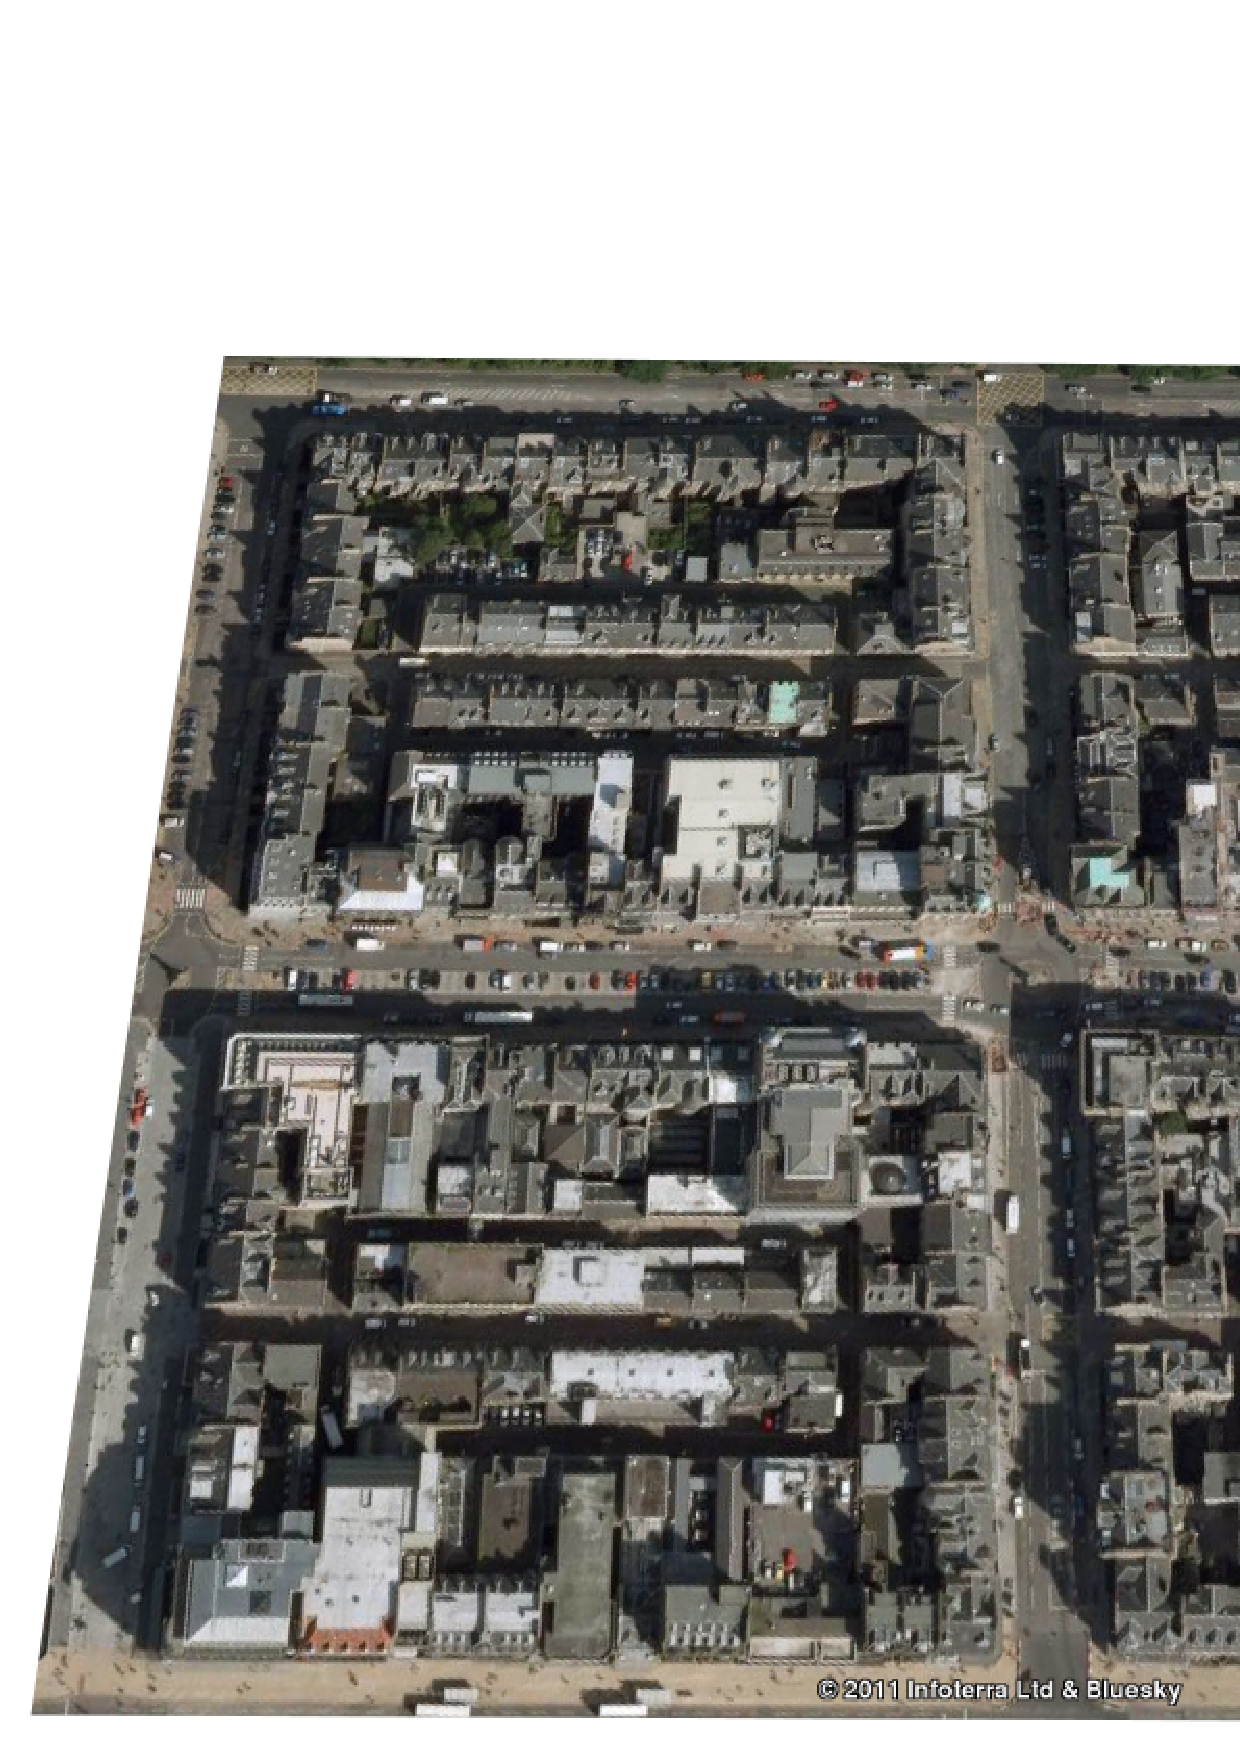
\includegraphics[width=0.8\linewidth]{fig/edinburgh.pdf} \\
Edinburgh, city centre. \\ 
$ 55^{\circ}57 ^{\backprime}16 ^{\backprime \backprime}  N  3^{\circ} 11 ^{\backprime} 58 ^{\backprime \backprime}  W $ \\
Elevation: $66 m$ \\
Area: $\approx 400 \times 300 m $
%%%%%%%%%%%%%%%%%%%%%%%%%%%%%%%%%%%%%%%%
\column{.1\textwidth}
\textit{... 1300 km away ...}
%%%%%%%%%%%%%%%%%%%%%%%%%%%%%%%%%%%%%%%%
\column{.43\textwidth}
\centering
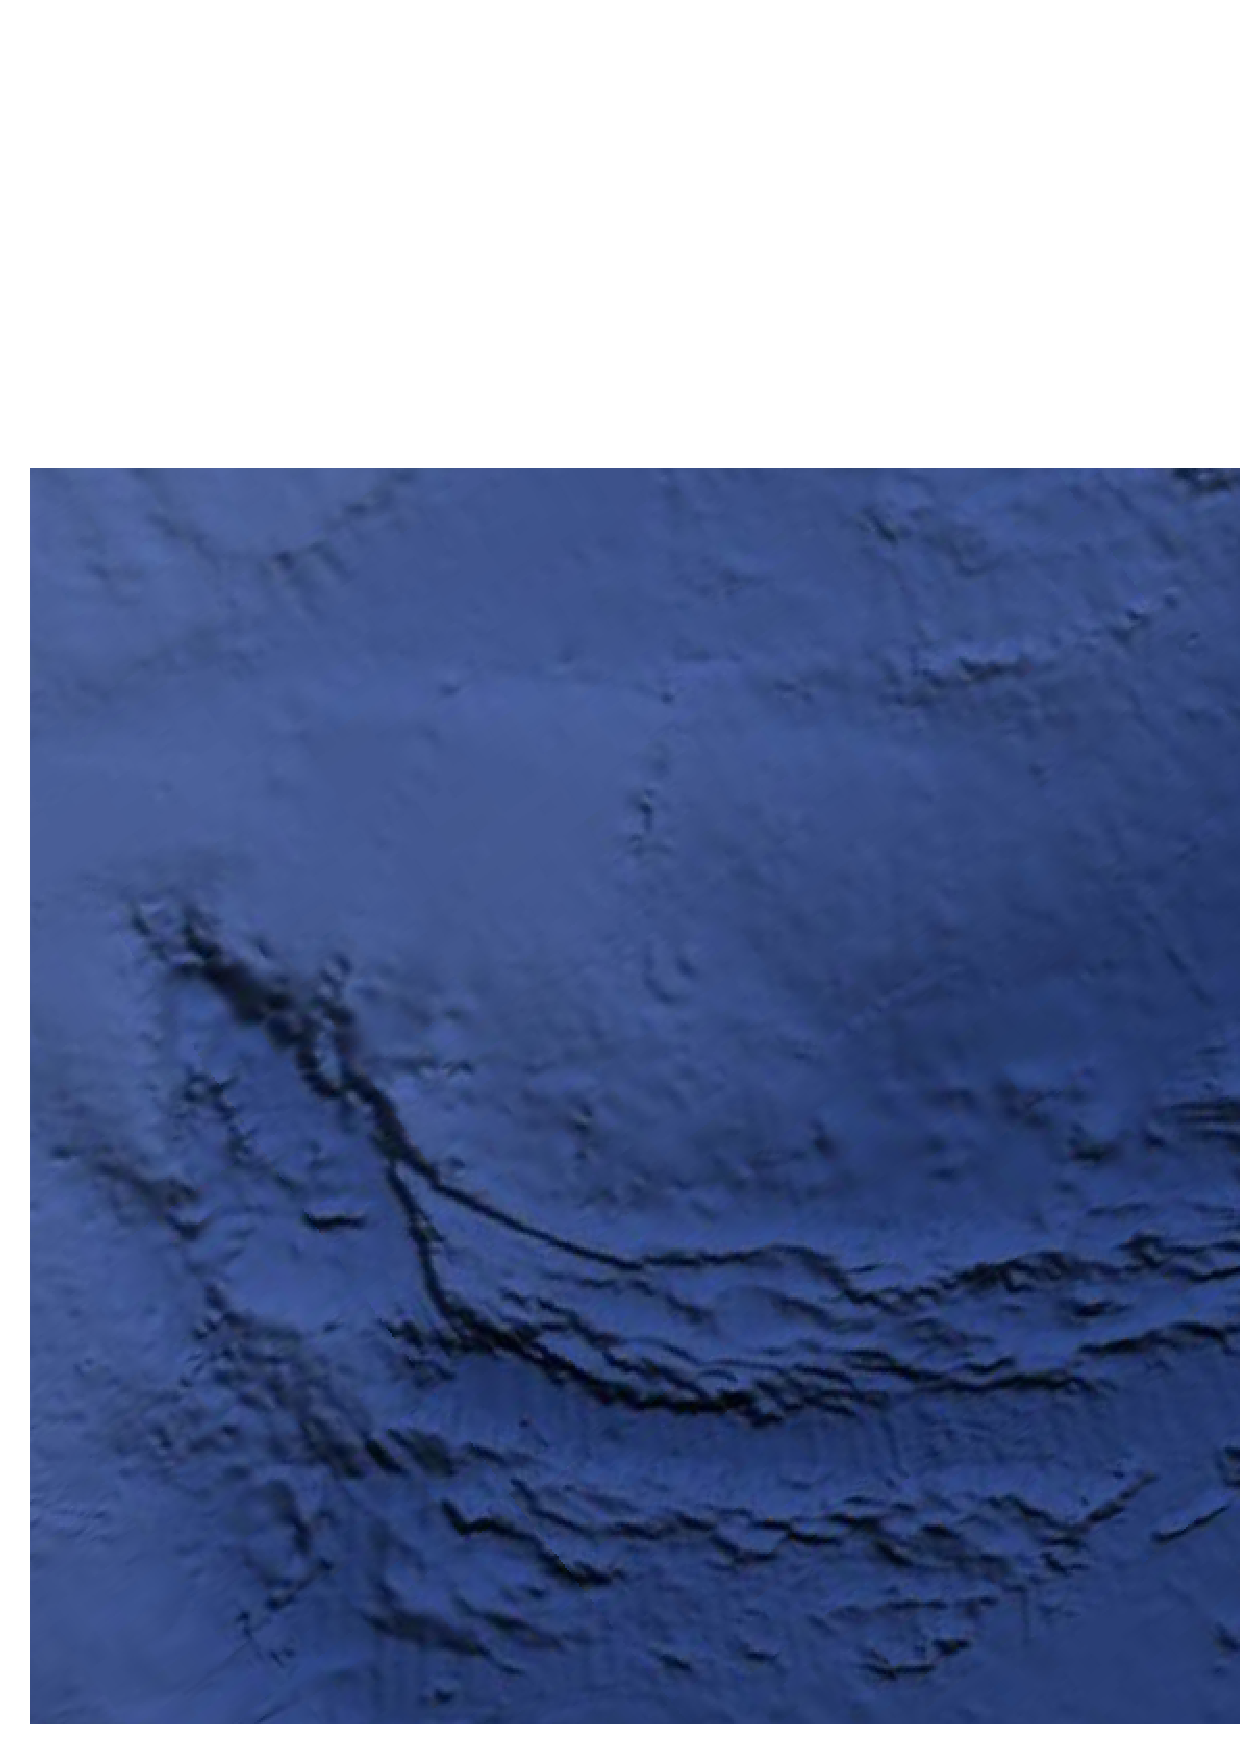
\includegraphics[width=0.8\linewidth]{fig/norwegianSea.pdf} \\
Norwegian sea. \\
$ 66^{\circ}  52 ^{\backprime} 46 ^{\backprime \backprime} N  3^{\circ}  36 ^{\backprime}  21 ^{\backprime \backprime} W $ \\
Elevation: $-3335 m$ \\
Area: $ \approx 700 \times 300 km $
\end{columns}
\end{block}

\begin{block} {Why navigation?}
	To be able to navigate the robot within the environment - we need to know it's position - to \textbf{localise} it.
\end{block}
%%mention applications: exploration, special tasks, mapping, inspections, military
\end{frame}

%%%%%%%%%%%%%%%%%%%%%%%%%%%%%%%%%%%%%%%%%%%%%%%%%%%%%%%%%%%%%%%%%%%%%%%%%%%%%%%

\begin{frame} \frametitle{Navigation}
\vspace{-10pt}
\textit{\textbf{Navigation}} implies the capabilities of:

{\footnotesize $\bullet$ accurate determination of the vehicle position and velocity with respect to a known reference point}

{\footnotesize $\bullet$ planning and the execution of the movements between locations}
\vspace{5pt}
\begin{columns}
\column{.4\textwidth}
\centering

\includegraphics[width=0.8\linewidth]{fig/map.pdf} \\
{\scriptsize John Harrison, $18^{th}$ century \\
\textit{longitude problem} }


\column{.2\textwidth}
\centering
\includegraphics[height=5em]{fig/phone-navigation.pdf} \\
{\scriptsize GPS, USDOD, 1974-1994. }

\column{.3\textwidth}
\centering
\includegraphics[height=5em]{fig/rov-navigation.pdf} \\
{\scriptsize  Underwater navigation strategies }
\end{columns} 
\vspace{5pt}
\hspace{0.5cm} \pro Measured depth is fairly accurate $\rightarrow$ localisation mainly 2d

\hspace{0.5cm} \contra Obtaining absolute position is more complex underwater

\hspace{0.5cm} \contra Cameras and sonar are of a limited use

\hspace{0.5cm} \contra Dead-reckoning sensors are expensive and prone to drifting

{\centering 
$\Longrightarrow$ use all available inertial information to navigate
}
\end{frame}

%%%%%%%%%%%%%%%%%%%%%%%%%%%%%%%%%%%%%%%%%%%%%%%%%%%%%%%%%%%%%%%%%%%%%%%%%%%%%%%

\chapter{Navigation sensors} \label{chap:sensors}

This chapter gives an overview of the sensors used in localization of an underwater vehicle and their characteristics.  Underwater positioning can be based on usage of different types of sensors together. Hence, it is possible to distinct localization that uses fixed, ground based reference, and relative positioning based on velocity integration. Localization is influenced with the development and performance sensor devices. Sensors can be regarded as the tool for managing the localization. Faster they are, more accurate they are, localization has more chances to perform better.

\section{Inertial navigation system}
Provides position, linear velocities, orientation and angular velocitioes. Accelerations are not used. 

\section{Acoustic system}
Provides the absolute position, ground-based reference. Principal way of exchanging the information through the environment is sound - therefore acoustic. Long baseline (LBL) is used for measuring position with respect to several tethered beacons placed in water (Section \S~\ref{sec:acoustic}). It can be understood as the extension of the GPS below the water surface. Such system uses acoustic signals to measure the distances. Vehicle uses the acoustic transponder to send the acoustic wave (``pinging''). The wave reaches beacon and reflects back to the vehicle. It consists of transceiver and array arranged collection of beacons. LBL transceiver pings each of the beacons and detects the signal travel time in order to calculate the distance. 

\section{Bathymetry system}
Accomplishes depth measurement. It is possible to use acoustic system for this purpose, however, bathymeter using pressure information tends to be more precise and trustable.

As stated in some practical implementations (\cite{blain03}), DVL and acoustic sensor perform 

\begin{itemize}
\item \textbf{DVL} - measures velocities
\item \textbf{COMPASS} - measures heading
\item \textbf{MRU} - in some robots used to measure roll and pitch
\end{itemize}

%%%%%%%%%%%%%%%%%%%%%%%%%%%%%%%%%%%%%%%%%%%%%%%%%%%%%%%%%%%%%%%%%%%%%%%%%%%%%%%

\begin{frame}\frametitle{Vehicle Navigation State Vector}
%The aim: accurate determination of the vehicle position and velocity
\begin{columns}
	\column{.62\textwidth}
	\textit{Vehicle state} is a vector that contains variables relevant for localising the vehicle (Eq. ~\ref{eq:state}). Vehicle navigation state describes its position and motion within the environment. Elements of the state vector $\vect{X}(k)$ are treated as Gaussian Random Variables (GRV). State vector will combine angular and metric values. \\
	{\footnotesize
	\begin{align}
		\vect{X}(k) = \left[ 
		\begin{array}{ccccccccccc}
		x & y & z & a & u & v & w & \psi & \varphi & \dot{\psi} & \dot{\varphi}
		\end{array} \right] ^{T}
		\label{eq:state}
	\end{align}
	}
{\footnotesize	
$\boldsymbol{x, y, z, a}$ : \textit{north}, \textit{east}, \textit{depth} and \textit{altitude} (Fig. \ref{fig:pos}). \\ 
$\boldsymbol{u, v, w}$ : linear velocities w.r.t sea bed in vehicle's coordinate system (\textit{surge}, \textit{sway} and \textit{heave}, Fig. \ref{fig:vel}) \\
$\boldsymbol{\psi, \varphi}$ : \textit{yaw} and \textit{pitch} (vehicle orientation, Fig. \ref{fig:pos}). \\
$\boldsymbol{\dot{\psi}, \dot{\varphi}}$ : \textit{yaw rate} and \textit{pitch rate} (angular velocities). 
} 
		
	\column{.35\textwidth}
	\begin{figure} %u, v, w - Velocity w.r.t sea bed in body coordinate
	\subfigure[velocities w.r.t. sea bed]{\label{fig:vel} 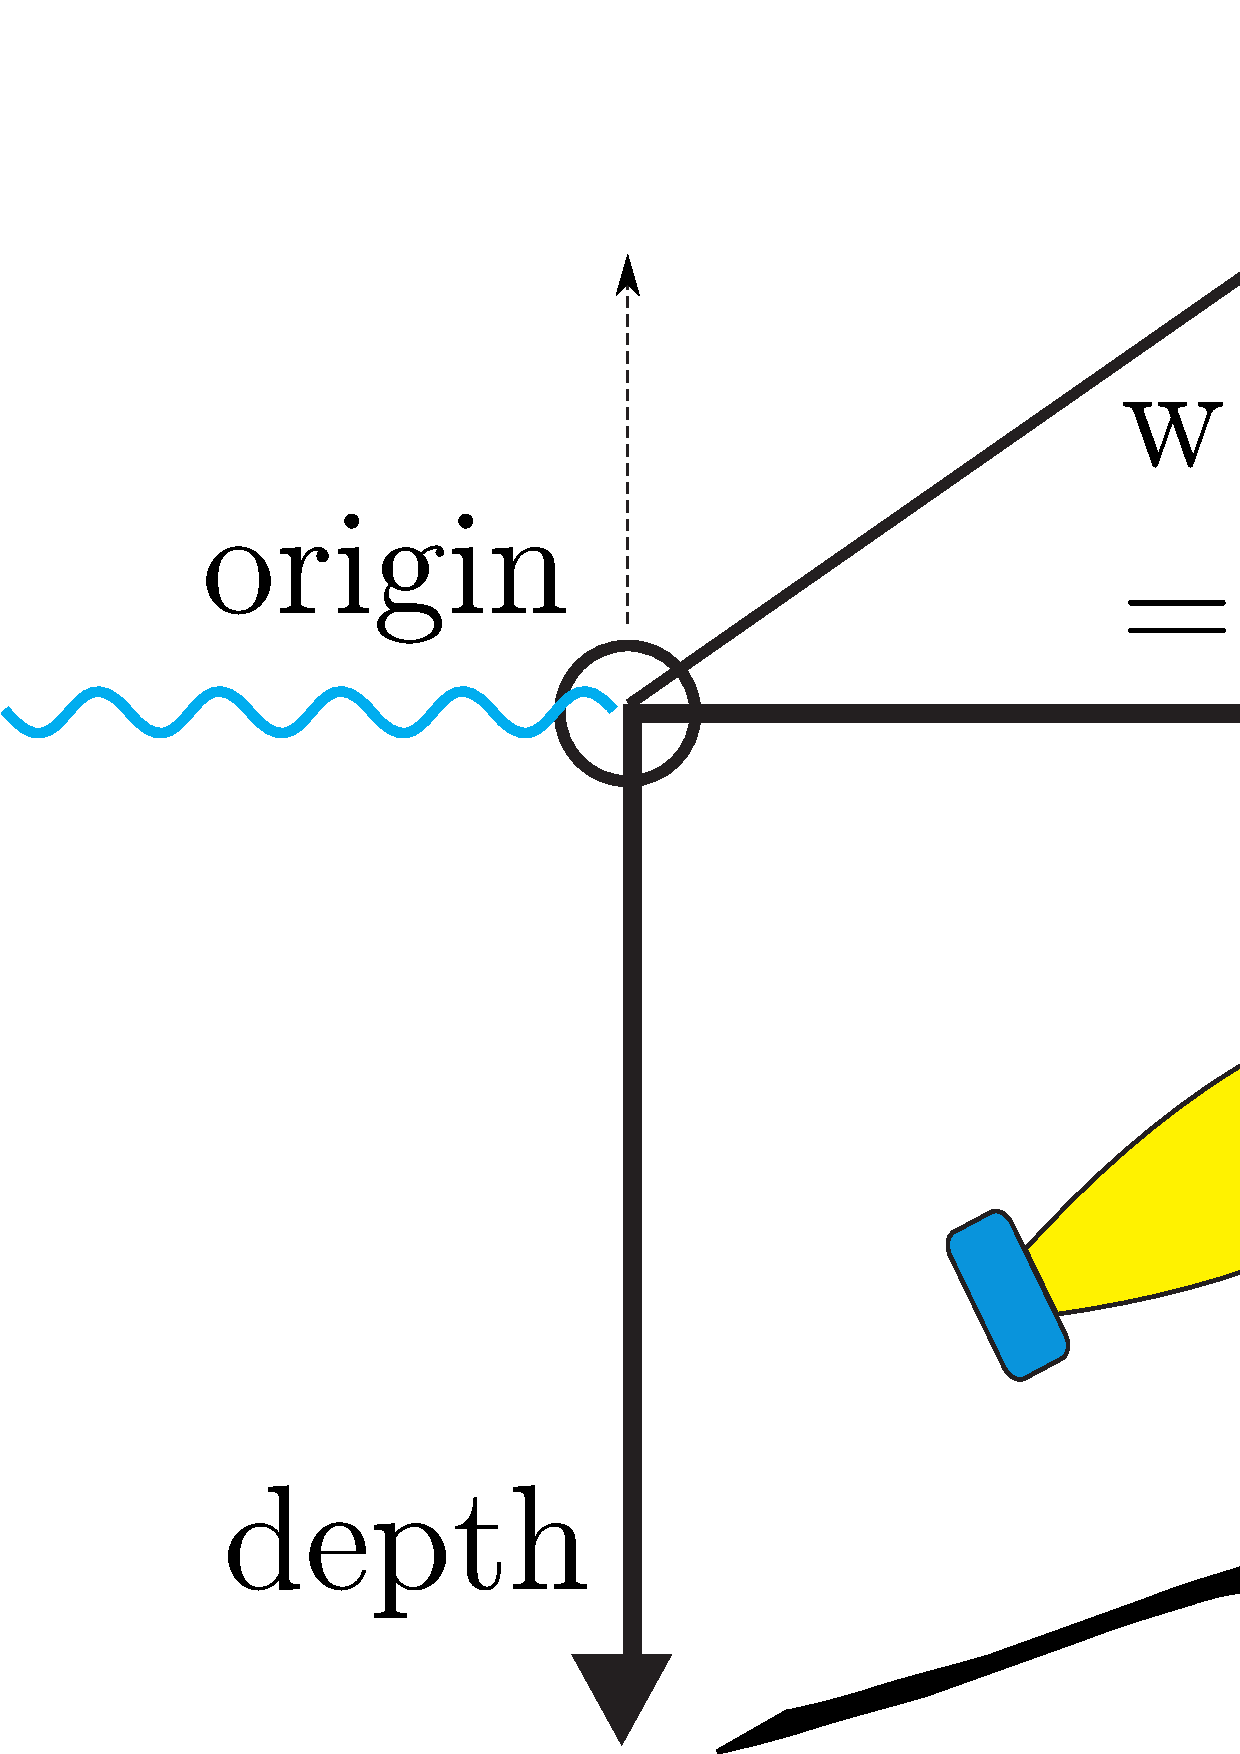
\includegraphics[width=0.95\linewidth]{fig/auv-axes.pdf}} \\
	\subfigure[global positioning]{\label{fig:pos} 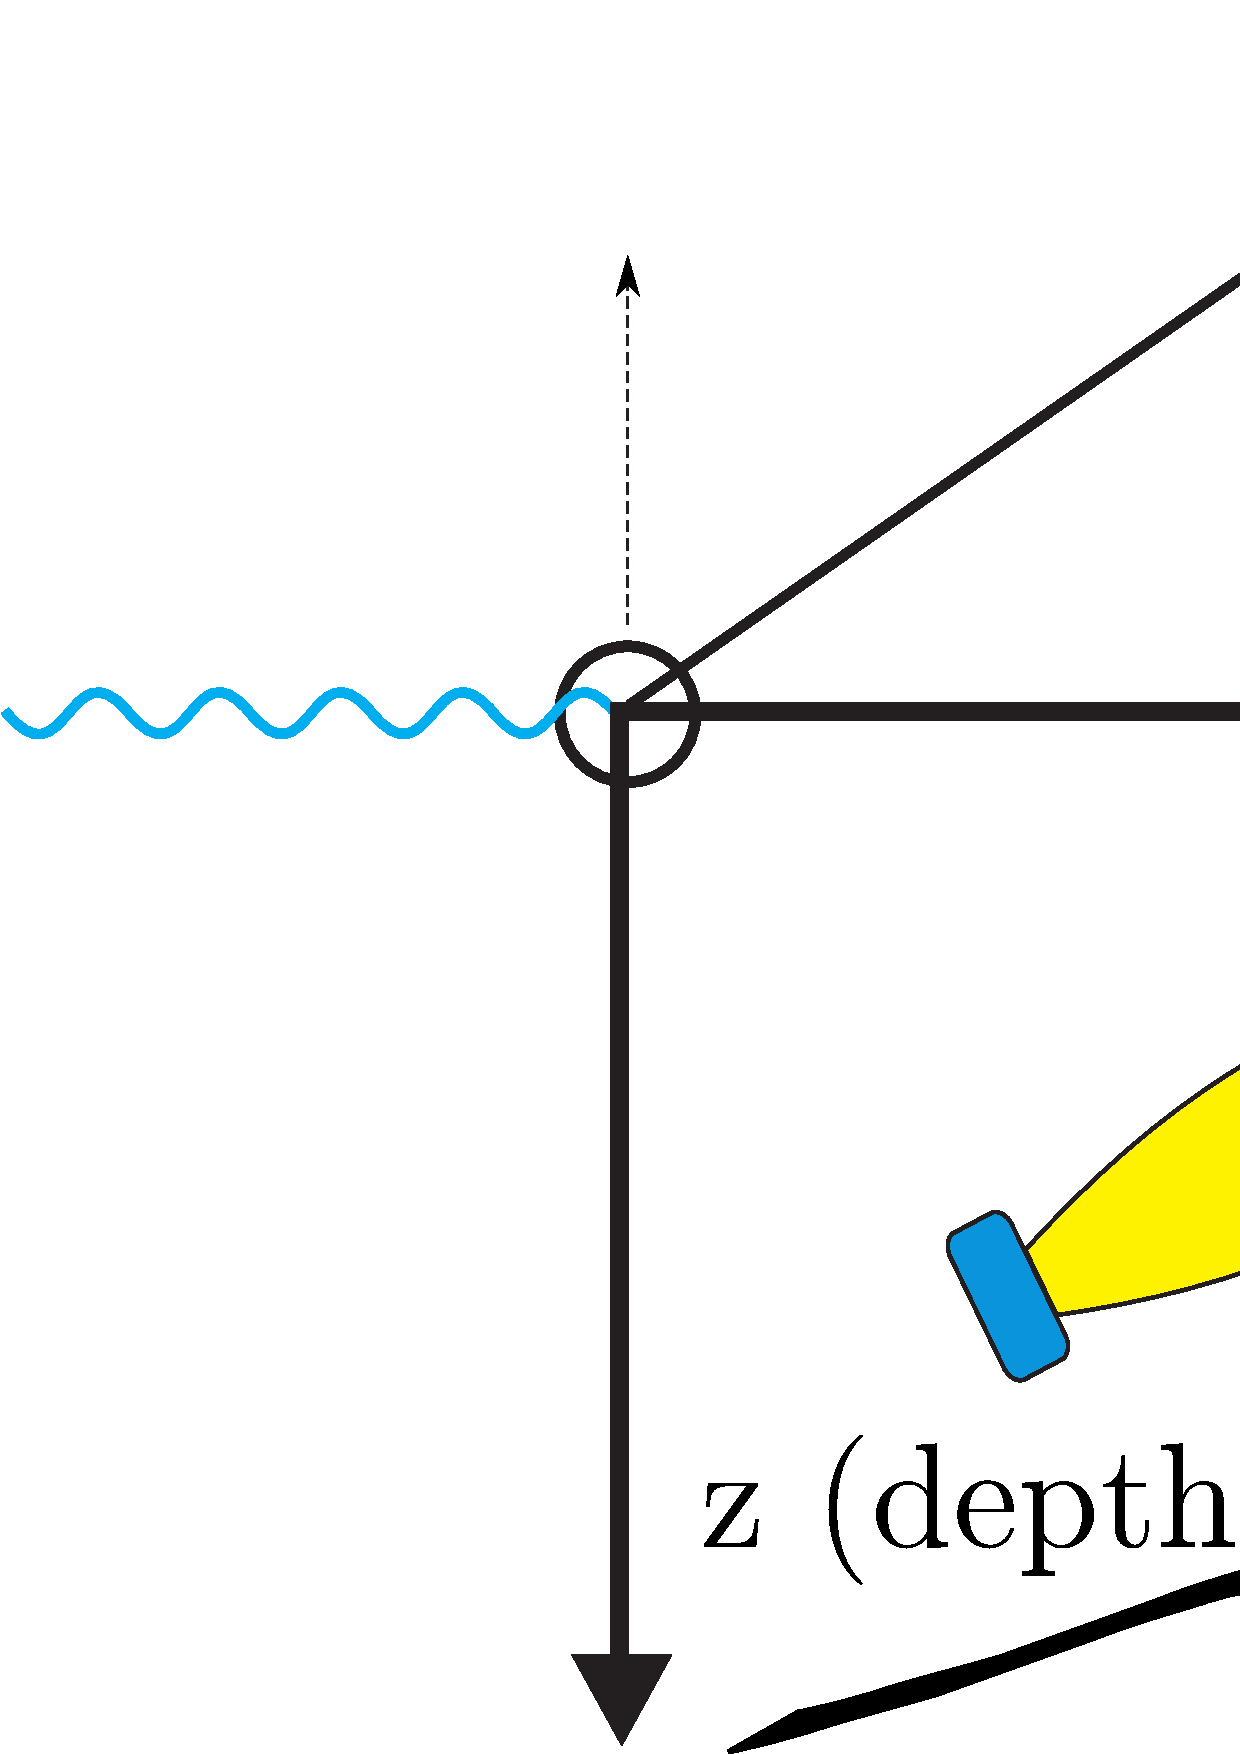
\includegraphics[width=0.95\linewidth]{fig/auv-model.pdf}}
	\caption{AUV positioning}
	\vspace{-25pt}
	\label{fig:positioning}
	\end{figure}
	
\end{columns}
\end{frame}



%%%%%%%%%%%%%%%%%%%%%%%%%%%%%%%%%%%%%%%%%%%%%%%%%%%%%%%%%%%%%%%%%%%%%%%%%%%%%%%

\begin{frame}\frametitle{System Model}
5 d.o.f. system model is describing how the state $\vect{X}(k)$ evolves in time. It is a \textit{constant speed} model \cite{ribas10} that uses previous state $\vect{X}(k-1)$ corrupted with \textit{zero-mean} GRV with linear and angular acceleration noise  $\vect{N}(k-1)$ to make a prediction of the next state vector value (Fig. ~\ref{fig:state-tran}, Eq. ~\ref{eq:state-tran}, ~\ref{eq:f}).
\begin{equation}
\vspace{-5pt}
\vect{X}(k) = f(\vect{X}(k-1), \vect{N}(k-1))
\label{eq:f}
\end{equation}
$$\vect{N}(k) = \left[ \begin{array}{ccccc} \dot{u} & \dot{v} & \dot{w} & \ddot{\psi} & \ddot{\varphi} \end{array} \right]^{T}$$% represents the process noise consisting of linear and angular accelerations.
\vspace{-10pt}
\begin{columns}
\column{.6\textwidth}
\begin{tiny}
\begin{equation}
\begin{bmatrix} x \\ y \\ z \\ a \\ \boldsymbol{u} \\ \boldsymbol{v} \\ \boldsymbol{w} \\ \psi \\ \varphi \\ \boldsymbol{\dot{\psi}} \\ \boldsymbol{\dot{\varphi}} \end{bmatrix}_{(k)} =
\begin{bmatrix} x + (uT+\dot{u}\frac{T^{2}}{2})\cos(\psi)\cos(\varphi) - (vT+\dot{v}\frac{T^{2}}{2})\sin(\psi)\cos(\varphi) \\ 
                y + (uT+\dot{u}\frac{T^{2}}{2})\sin(\psi)\cos(\varphi) + (vT+\dot{v}\frac{T^{2}}{2})\cos(\psi)\cos(\varphi) \\ 
                z + (wT+\dot{w}\frac{T^{2}}{2})\cos(\varphi) \\ 
                a - (wT+\dot{w}\frac{T^{2}}{2})\cos(\varphi) \\ 
                \boldsymbol{u} + \dot{u}T \\ 
                \boldsymbol{v} + \dot{v}T \\ 
                \boldsymbol{w} + \dot{w}T \\ 
                \psi    + \dot{\psi}T    + \ddot{\psi}   \frac{T^{2}}{2} \\ 
                \varphi + \dot{\varphi}T + \ddot{\varphi}\frac{T^{2}}{2} \\ 
                \boldsymbol{\dot{\psi}}    + \ddot{\psi}T \\ 
                \boldsymbol{\dot{\varphi}} + \ddot{\varphi}T
\end{bmatrix}_{(k-1)} 
\label{eq:state-tran}
\end{equation} %% defined as zero-mean GRV.
\end{tiny}
\column{.35\textwidth}
\begin{figure}
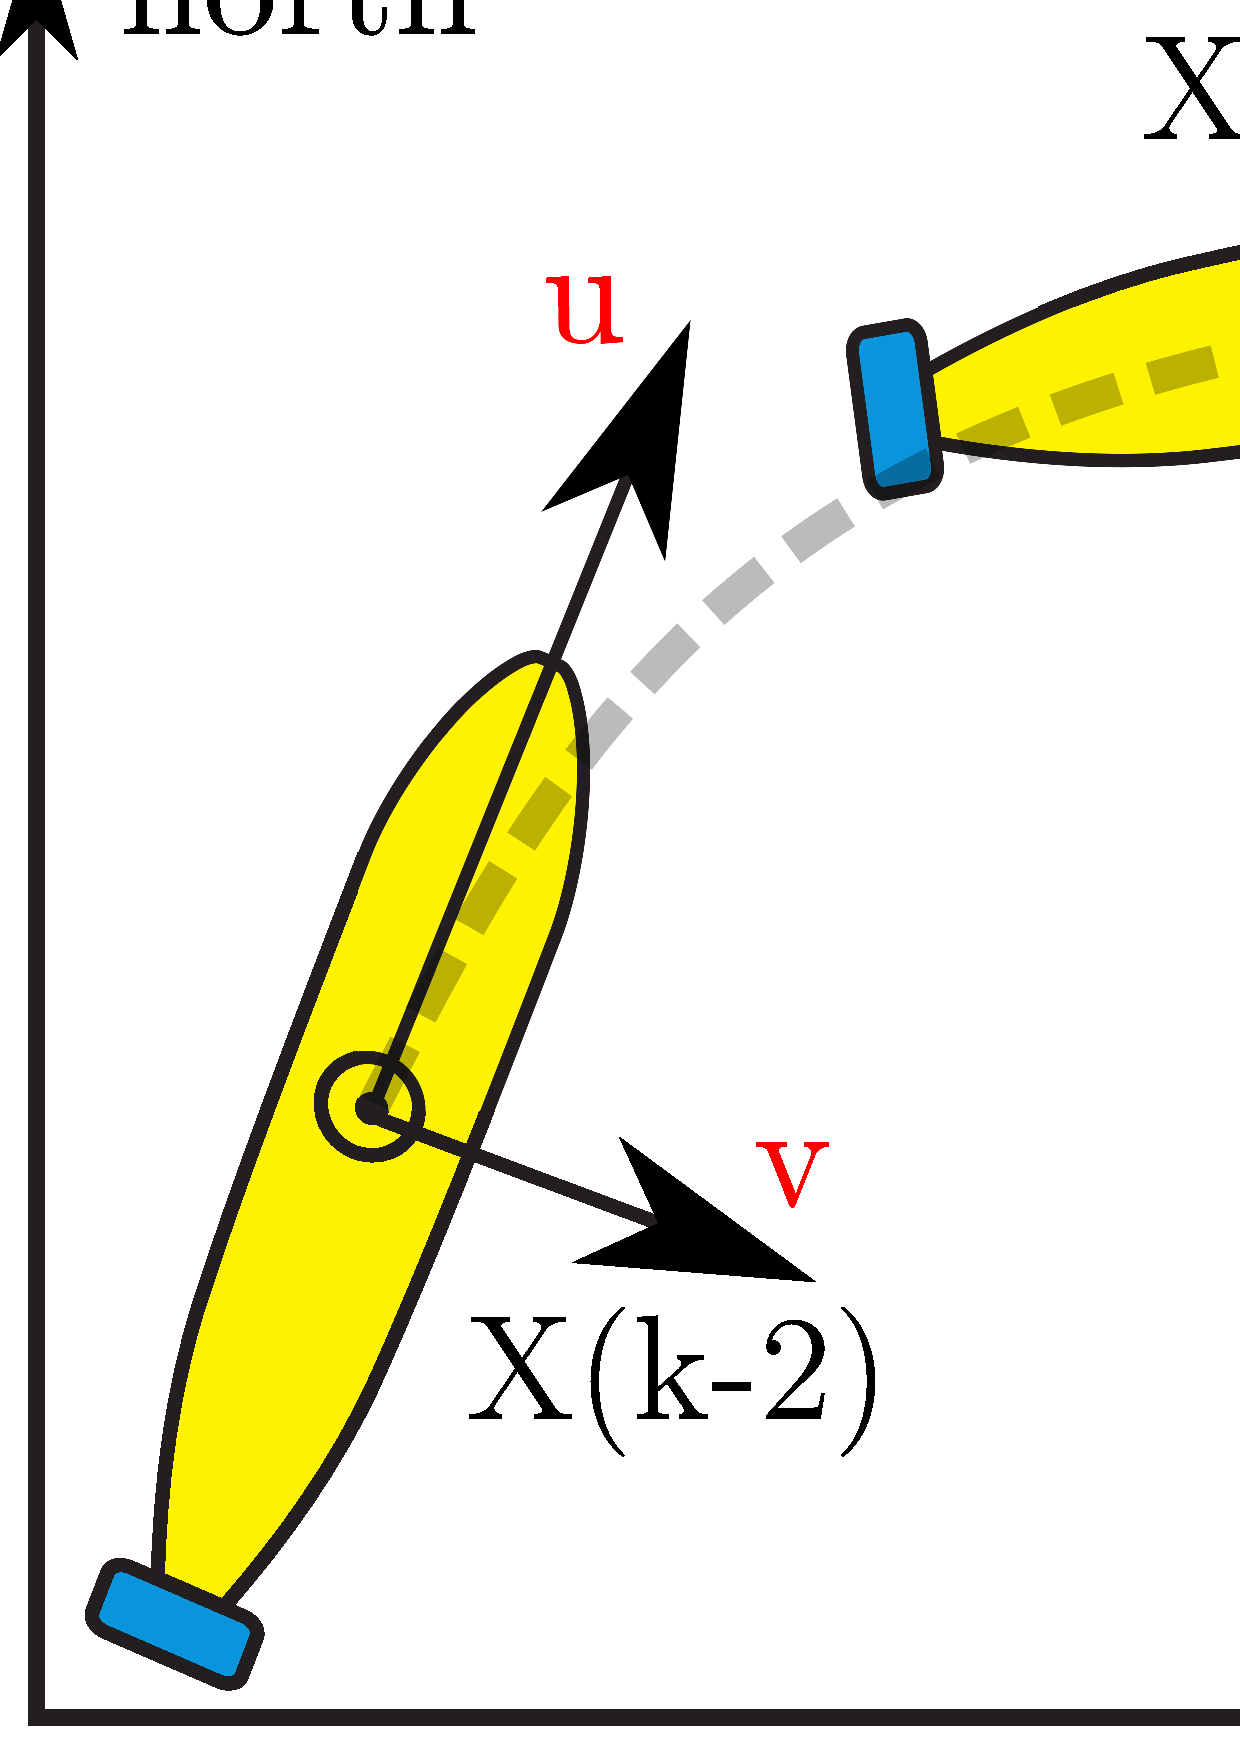
\includegraphics[width=0.98\linewidth]{fig/model.pdf}
\caption{{\scriptsize State transition model}}
\label{fig:state-tran}
\end{figure}
\end{columns}
\end{frame}

%%%%%%%%%%%%%%%%%%%%%%%%%%%%%%%%%%%%%%%%%%%%%%%%%%%%%%%%%%%%%%%%%%%%%%%%%%%%%%%

\begin{frame}\frametitle{Extended Kalman Filter (EKF)}%estimating the state of a nonlinear dynamic system
The goal is to estimate the vehicle state $\vect{X}(k)$ using sensor measurements $\vect{Z}(k)$, process $\vect{N}(k-1)$ and measurement $\vect{M}(k)$ noise. \\
\begin{columns}
	\column{.45\textwidth}
	\begin{block}{How does it work?}
	\centering
	
\includegraphics[width=0.85\linewidth]{fig/diagram-kalman.pdf}
	\end{block} 
\vspace{-25pt}	
	\begin{equation*} 
	\vect{X}(k) = f(\vect{X}(k-1), \vect{N}(k-1)) \; prediction
	\end{equation*}
\vspace{-25pt}	
	\begin{equation*}
	\vect{Z}(k) = h(\vect{X}(k), \vect{M}(k))  \; measurement%= \vect{H} \vect{X}(k \mid k-1)  + \vect{M}(k)
	\end{equation*}

\column{.45\textwidth}
\vspace{-5pt}
	\begin{itemize}
		\item \begin{footnotesize}``standard'' in nonlinear estimation, \textit{Bayesian} approach\end{footnotesize} %used in other applications - GPS, nav
		%\item \begin{footnotesize}\end{footnotesize}   % involving computing posterior PDF 
		\item \begin{footnotesize}$1^{st}$ order Taylor expansion of the nonlinear functions \end{footnotesize} 
		\item \begin{footnotesize}provides estimation uncertainties in form of error covariance matrices \end{footnotesize} 
		\item \begin{footnotesize}difficult tuning \end{footnotesize}
		\item \begin{footnotesize}reliable for systems that are almost linear on the time scale of the updates \end{footnotesize}
	\end{itemize}	
	%\begin{block}{Interesting alternative: Unscented Kalman Filter}
	%\end{block}
\end{columns}
\end{frame}

%%%%%%%%%%%%%%%%%%%%%%%%%%%%%%%%%%%%%%%%%%%%%%%%%%%%%%%%%%%%%%%%%%%%%%%%%%%%%%%

\begin{frame}\frametitle{Interesting alternative: Unscented Kalman Filter (UKF)}
The goal stays the same: to estimate the state $\vect{X}(k)$: mean ($\hat{X}$) and covariance ($P$). %Framework is similar: Nonlinear filter that does \textit{prediction \& correction}, uses Bayesian approach. \\
\vspace{-5pt}
\begin{columns}
	\column{.45\textwidth}
	\begin{block}{e.g. Mapping from Polar to Cartesian coordinates}
	\centering
	\begin{figure}
	\subfigure[{\scriptsize polar coord.}]{\includegraphics[width=0.45\linewidth]{fig/orig.pdf}}
	\subfigure[{\scriptsize $\hat{X}, P$ (EKF)}]{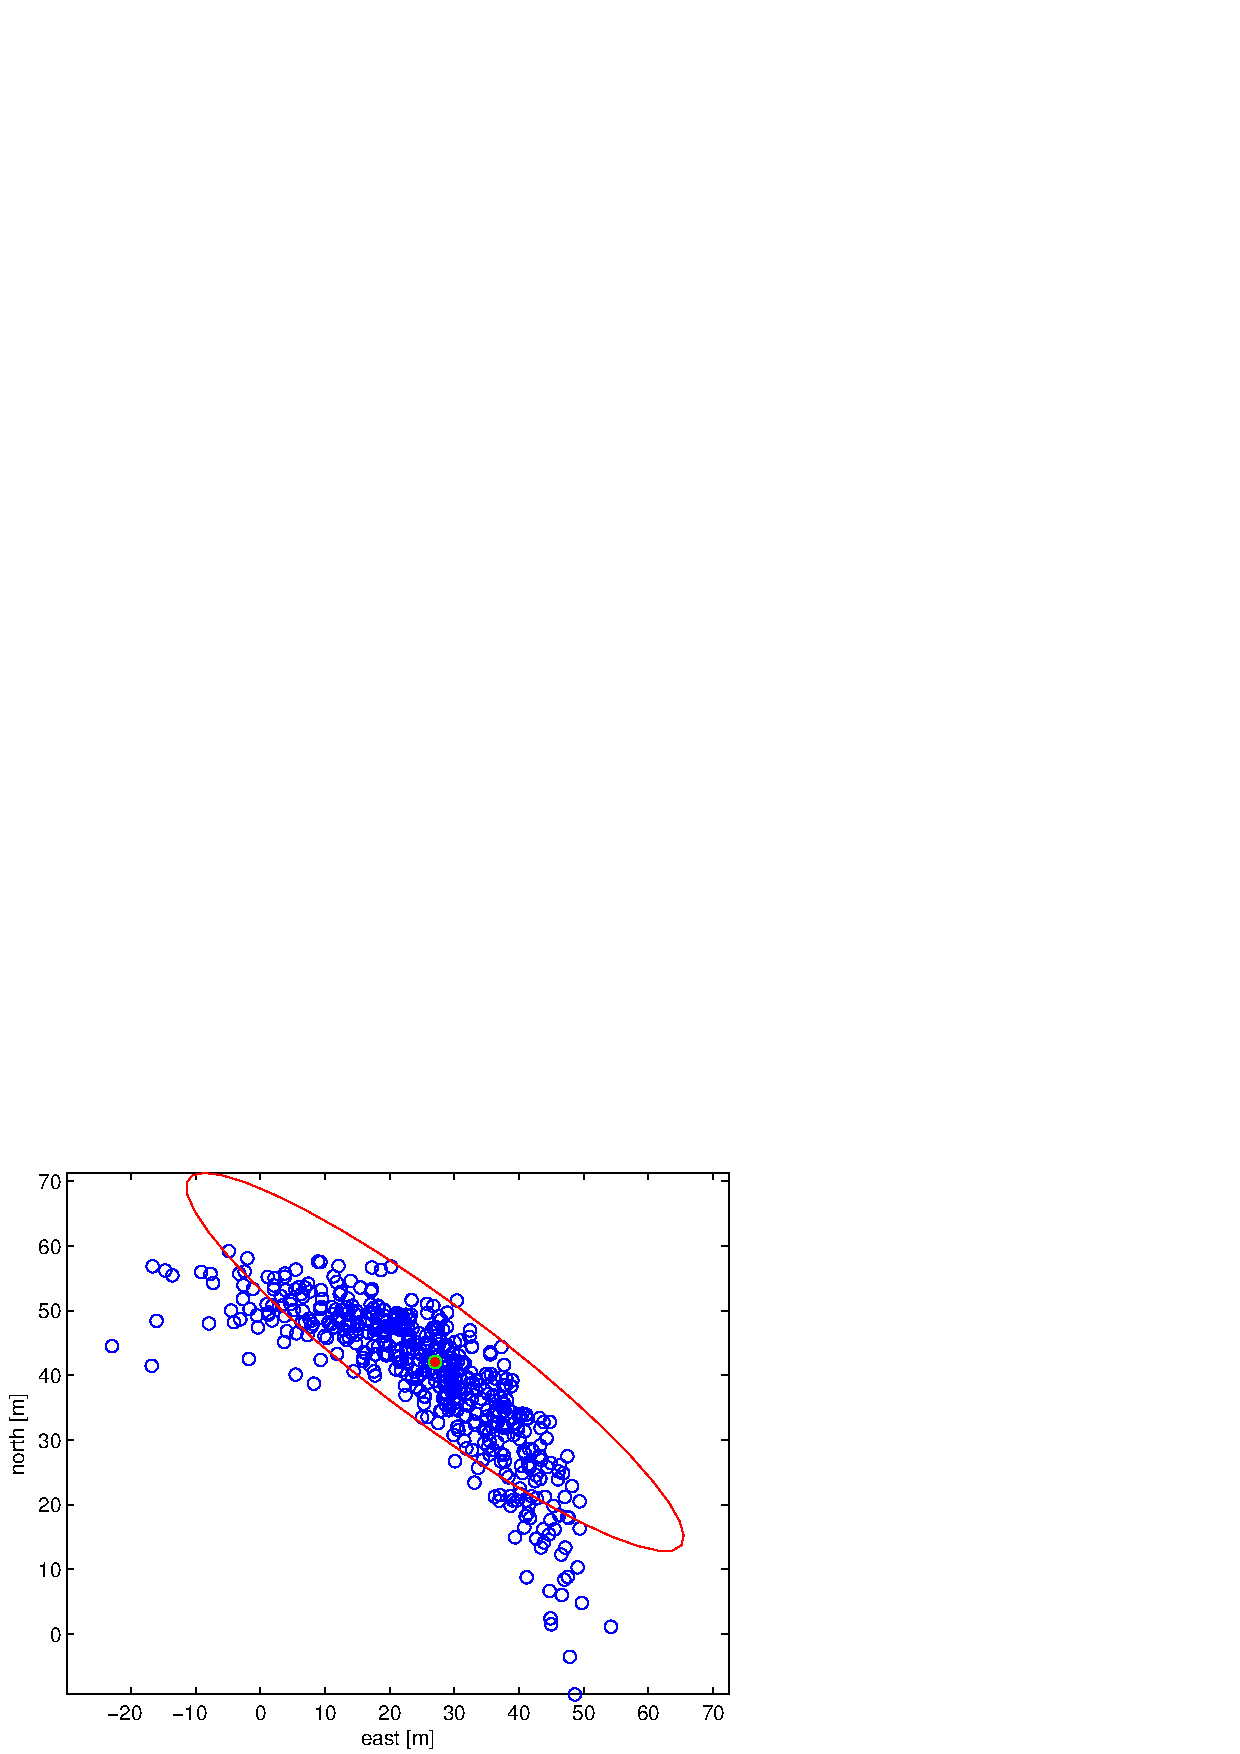
\includegraphics[width=0.45\linewidth]{fig/linear.pdf}} \\
	\subfigure[{\scriptsize UT sampled}]{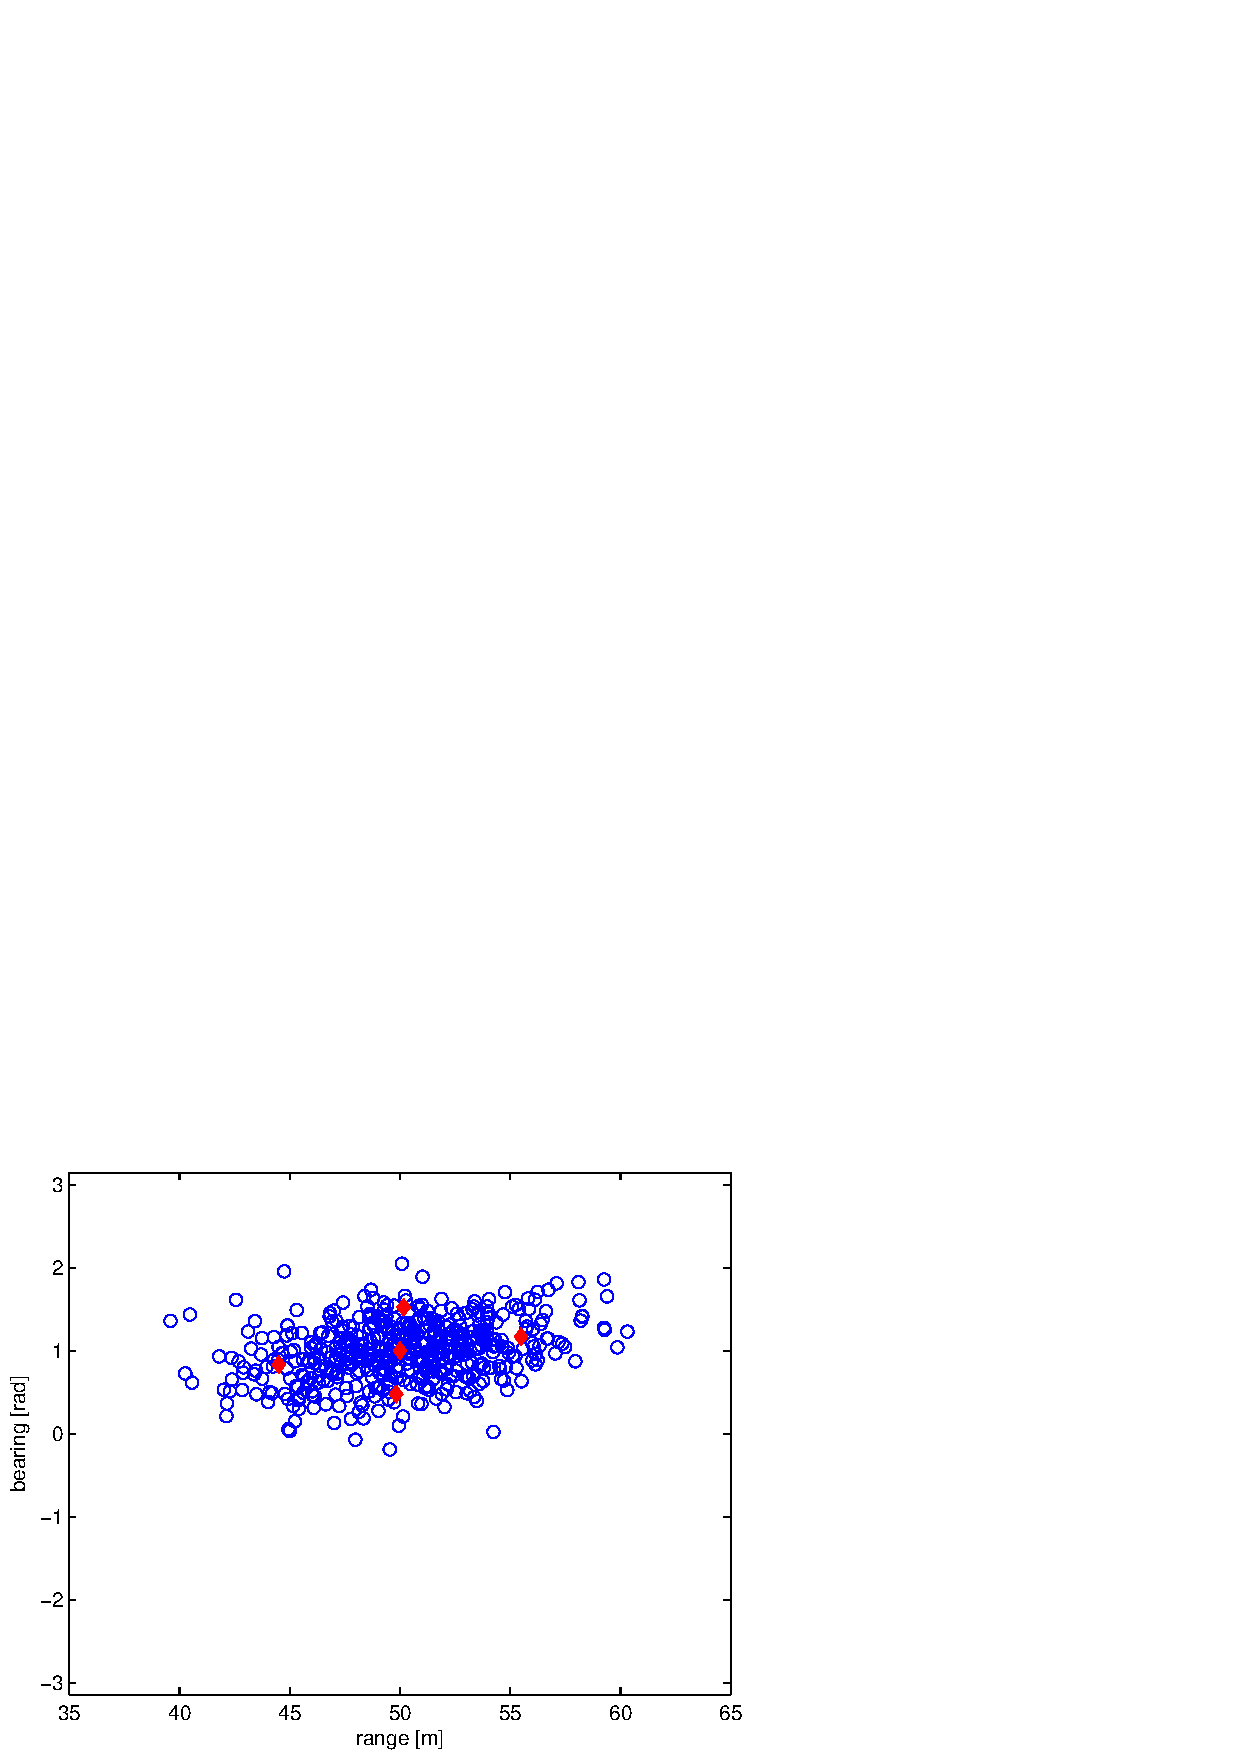
\includegraphics[width=0.45\linewidth]{fig/orig-samples.pdf}}
	\subfigure[{\scriptsize $\hat{X}, P$ (UKF)}]{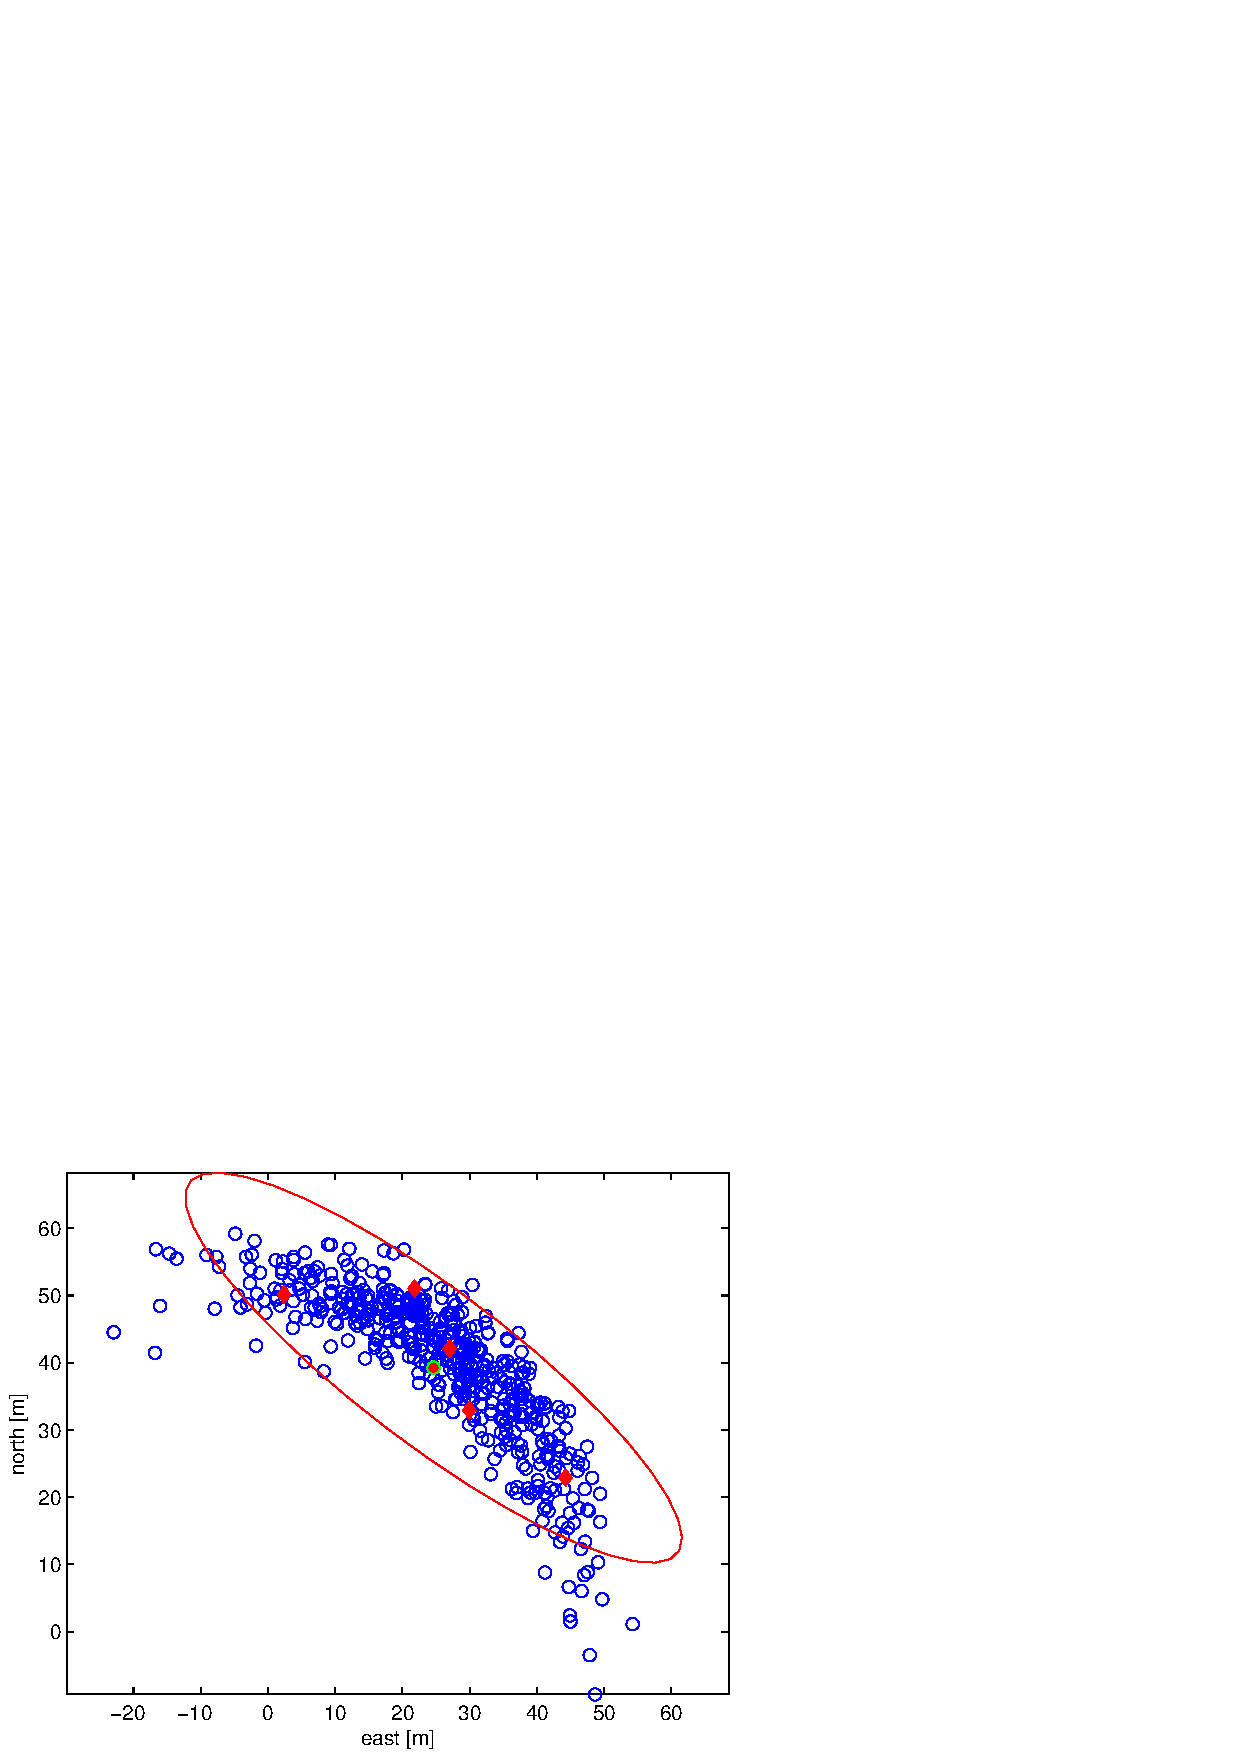
\includegraphics[width=0.45\linewidth]{fig/unscented.pdf}} \\
	\end{figure}
	\end{block} 

\column{.48\textwidth}
%\centering 
\vspace{-10pt}
\begin{columns}
\column{.38\textwidth}
\begin{block}{EKF}
{\scriptsize linearisation of the transform}
\end{block}
%\textbf{EKF} \\
%
\column{.58\textwidth}
\begin{block}{UKF}
{\scriptsize pdf is estimated using a collection of samples of a GRV propagated through the nonlinear transformation}
\end{block}
%\textbf{UKF} \\
%
\end{columns}
\vspace{5pt}
\textbf{Unscented Transform} (UT): selects the samples of a Gaussian and assigns a weight to each. 
	\begin{itemize}
		\item {\footnotesize guarantees $2^{nd}$ order Taylor expansion accuracy \cite{julier96}} 
		\item {\footnotesize no infamous Jacobians} 
		\item {\footnotesize same computational cost as EKF} 
	\end{itemize}	
\end{columns}
\end{frame}

%%%%%%%%%%%%%%%%%%%%%%%%%%%%%%%%%%%%%%%%%%%%%%%%%%%%%%%%%%%%%%%%%%%%%%%%%%%%%%%

\begin{frame}\frametitle{Sensor Fusion}%EKF implements sensor fusion. 
Sensor measurements are not available all the time - messages from sensors arrive at different moments and sensors could be unavailable due to different causes. 
\vspace{-5pt}
\begin{columns}
\column{.7\textwidth}
	\center{
    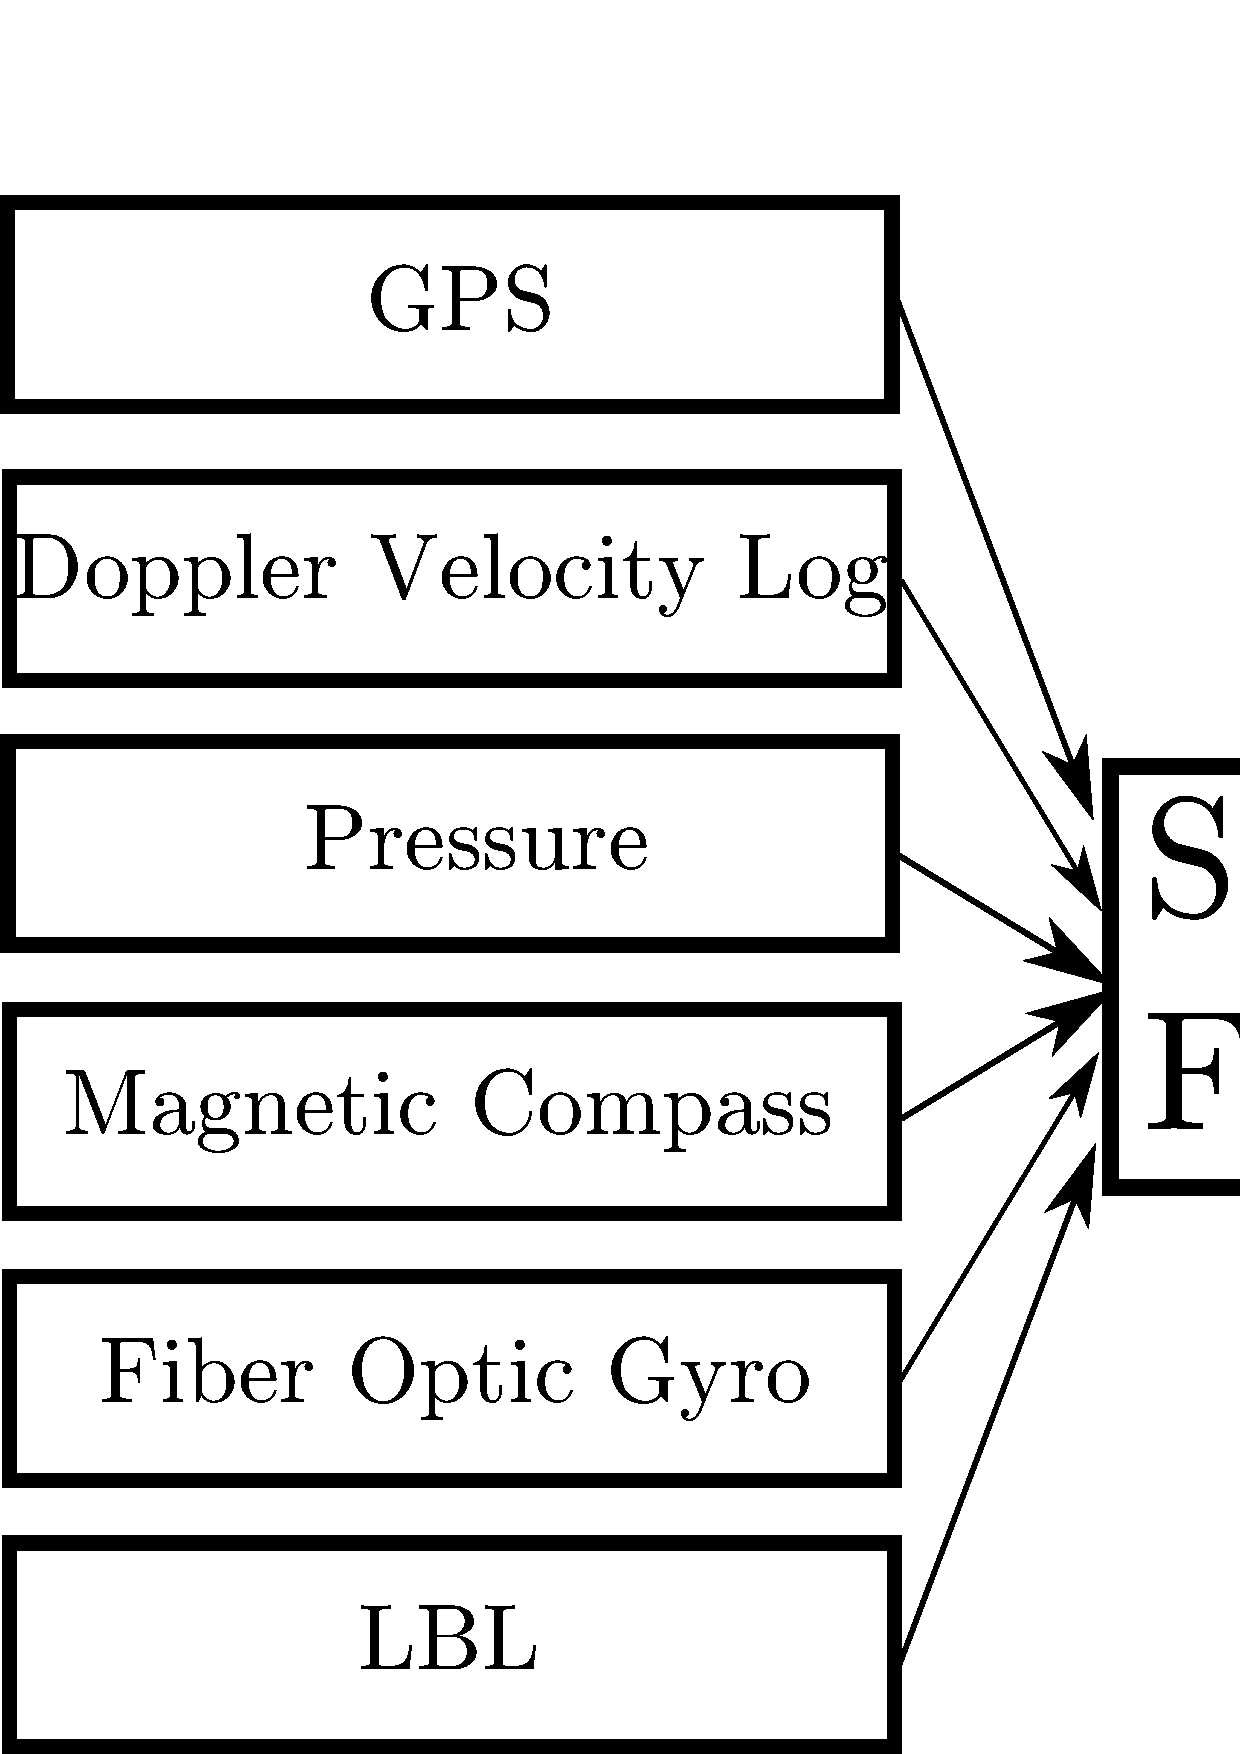
\includegraphics[width=0.98\linewidth]{fig/fusion-all.pdf}} \\
	\vspace{-5pt}
\hspace{3em} 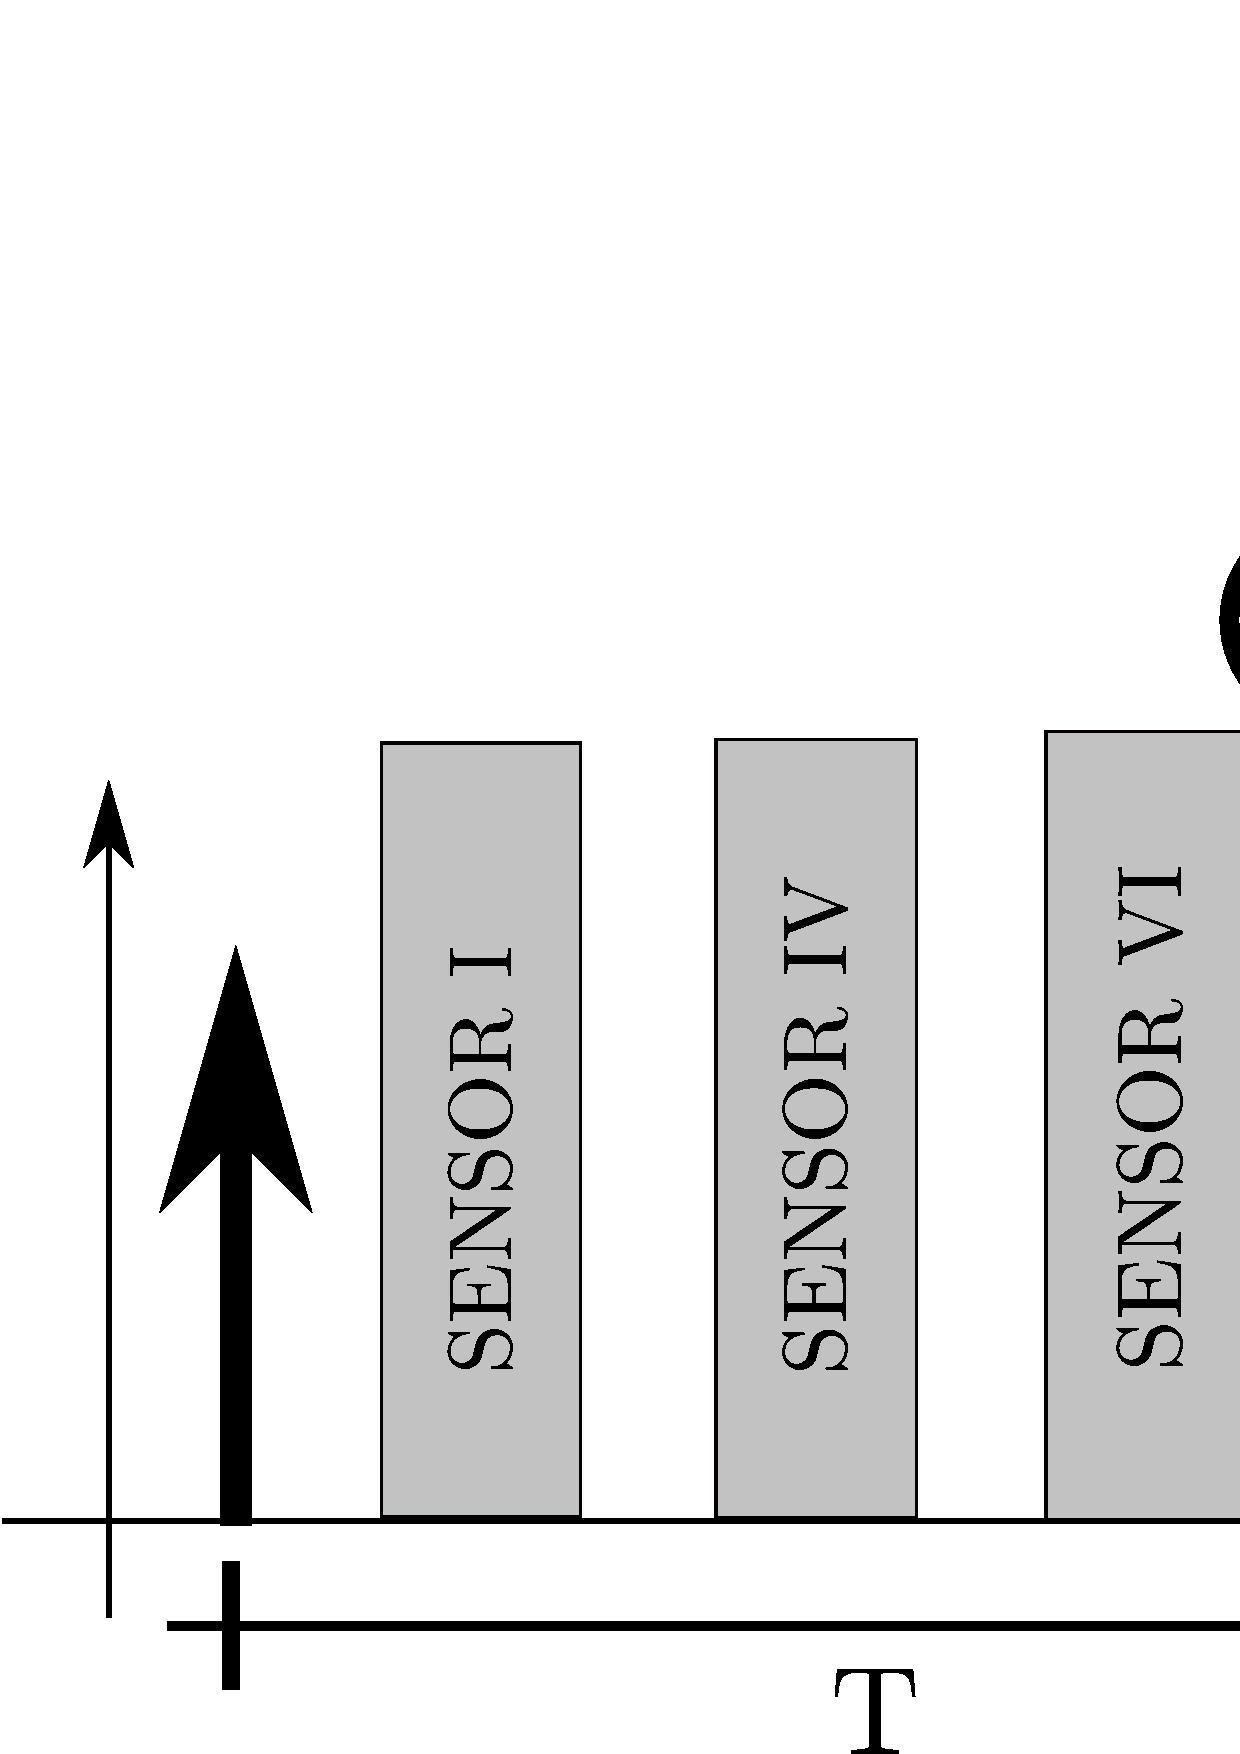
\includegraphics[width=0.43\linewidth]{fig/synch.pdf} 
\column{.28\textwidth}
	Gather the information in between the cycles and integrate it together in the measurement model (Eq. ~\ref{eq:fuse}).%, which varies depending on the measured values and sensors used for the measurement.
\end{columns}	
\begin{equation}
\label{eq:fuse}
\vect{Z}(k) = \left[ \begin{array}{c} \vect{Z}_{sen. I} \\ \vect{Z}_{sen. II}  \end{array} \right],
\vect{H}(k) = \left[ \begin{array}{c} \vect{H}_{sen. I} \\ \vect{H}_{sen. II}  \end{array} \right], 
\vect{R}(k) = \left[ \begin{array}{cc} \vect{R}_{sen. I} & 0 \\ 0 & \vect{R}_{sen. II} \end{array} \right]
\end{equation}
\vspace{-10pt}	
	\begin{equation*}
	\vect{Z}(k) = h(\vect{X}(k), \vect{M}(k)) = \vect{H} \vect{X}(k \mid k-1)  + \vect{M}(k)
	\end{equation*}
%parameters 
$\vect{R}_{sen. I}$ and $\vect{R}_{sen. II}$ are defining sensor measurement (un)certainty.
\end{frame}

%%%%%%%%%%%%%%%%%%%%%%%%%%%%%%%%%%%%%%%%%%%%%%%%%%%%%%%%%%%%%%%%%%%%%%%%%%%%%%%

\begin{frame}\frametitle{Why Kalman?}
\begin{columns}[t]
\column{.49\textwidth}
\textbf{I. Blending the measurements}\\ %\begin{block}{}
\vspace{-1em}
\begin{center}
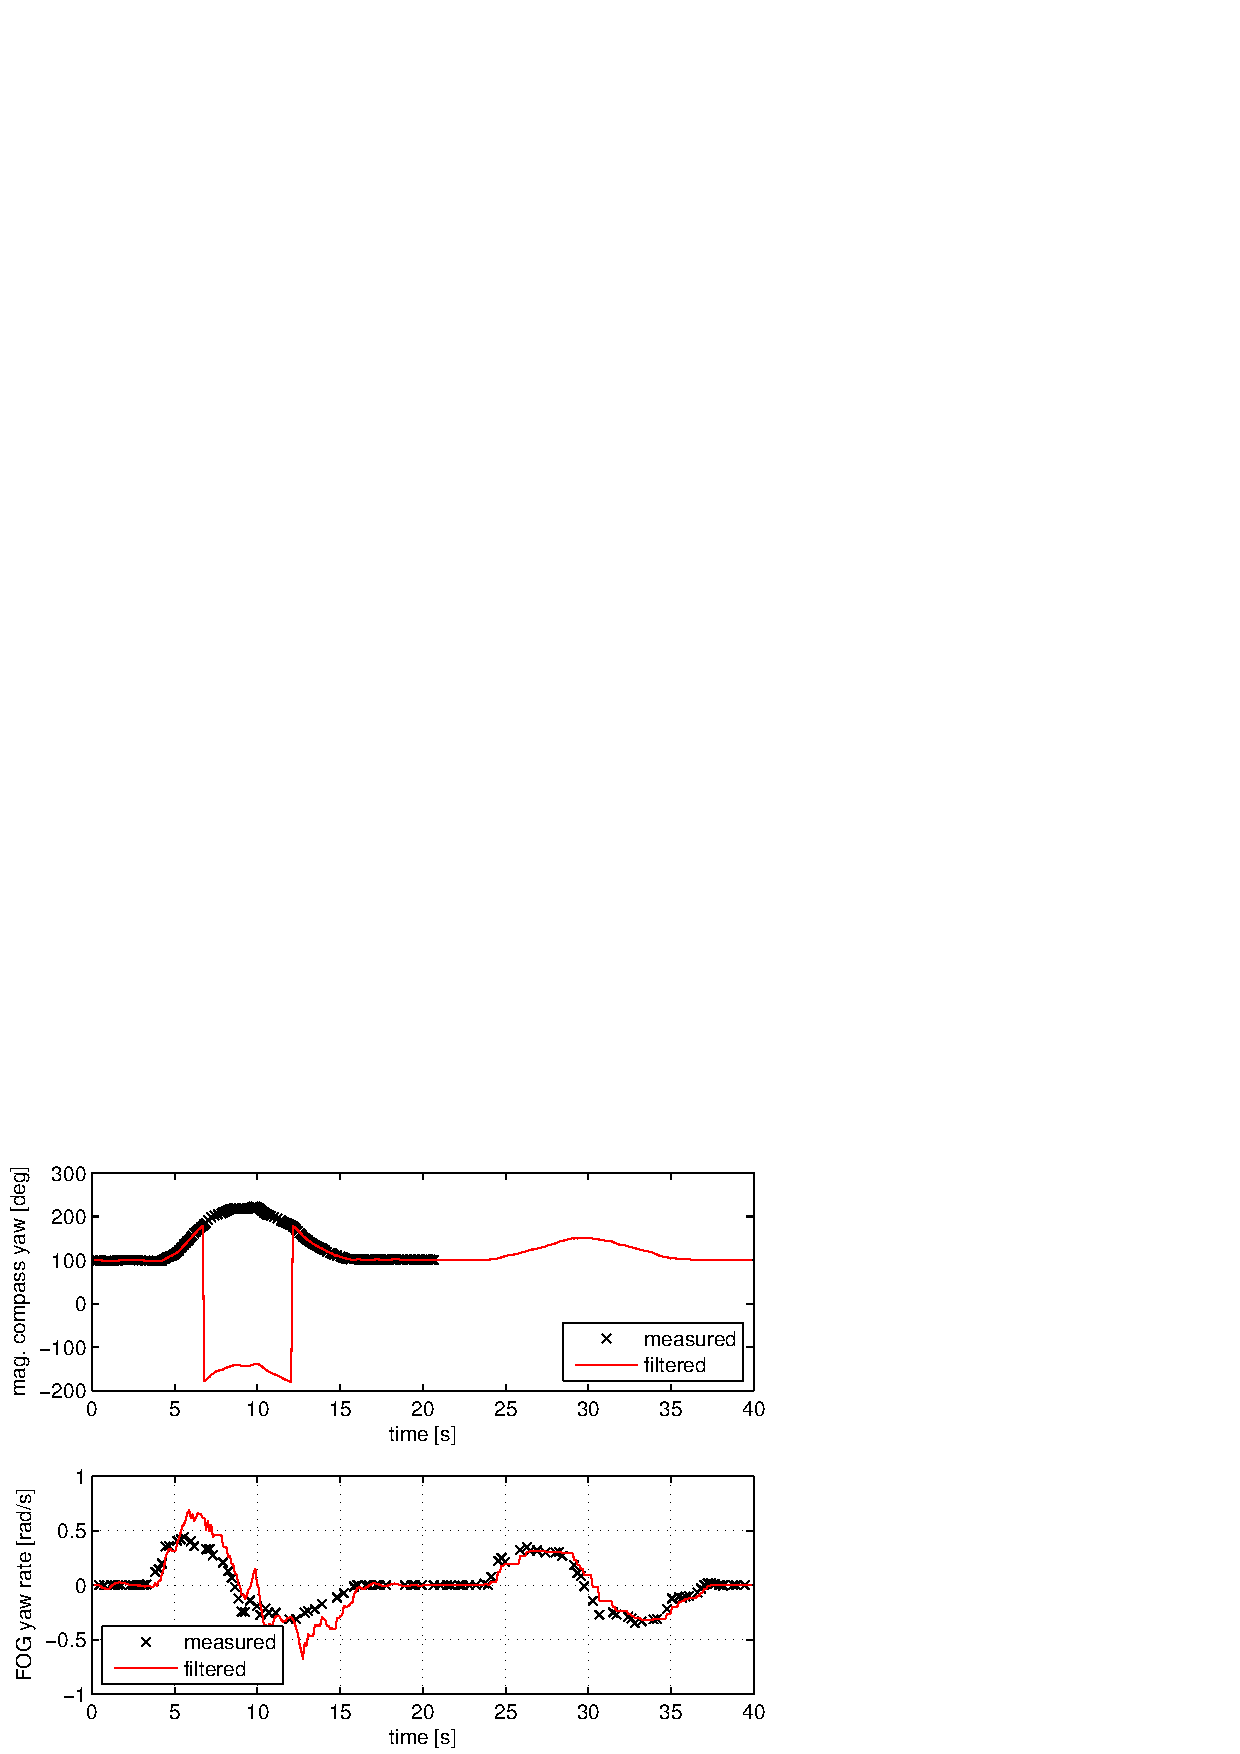
\includegraphics[width=0.8\linewidth]{fig/lostCompass.pdf}
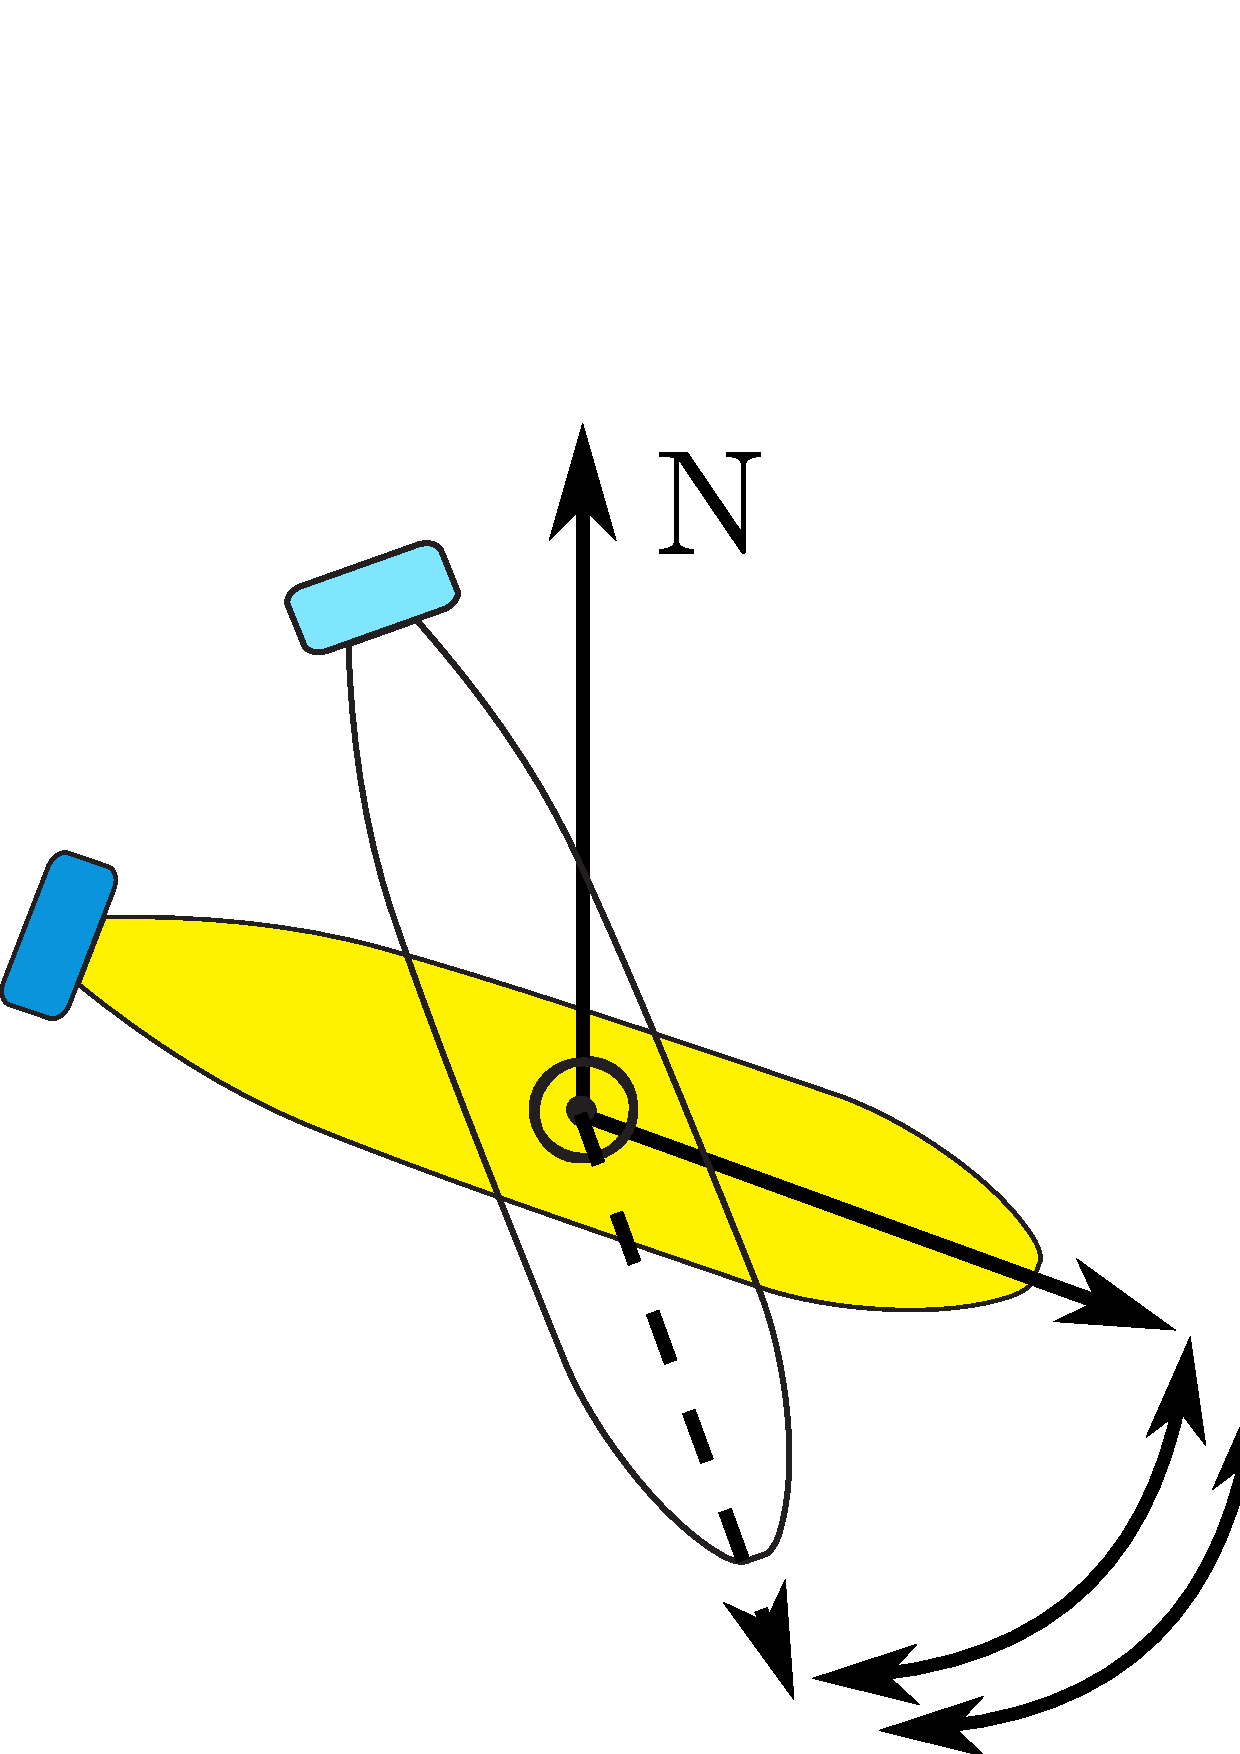
\includegraphics[width=0.19\linewidth]{fig/rotate.pdf} \\
\end{center}
\vspace{-1em}
yaw $(\psi)$ is inferred from compass \& FOG.\\
\textit{EKF benefit}: \pro if one of them stops working - the other one tries to compensate the failure

			\column{.49\textwidth}%$\Rightarrow$ 
			\textbf{II. Prediction \& Filtering} \\ %\begin{block}{}
			If the measurement temporarily fails, EKF keeps predicting. Noisy velocity information is filtered. \\%, with increased uncertainty. \\
			\centering
			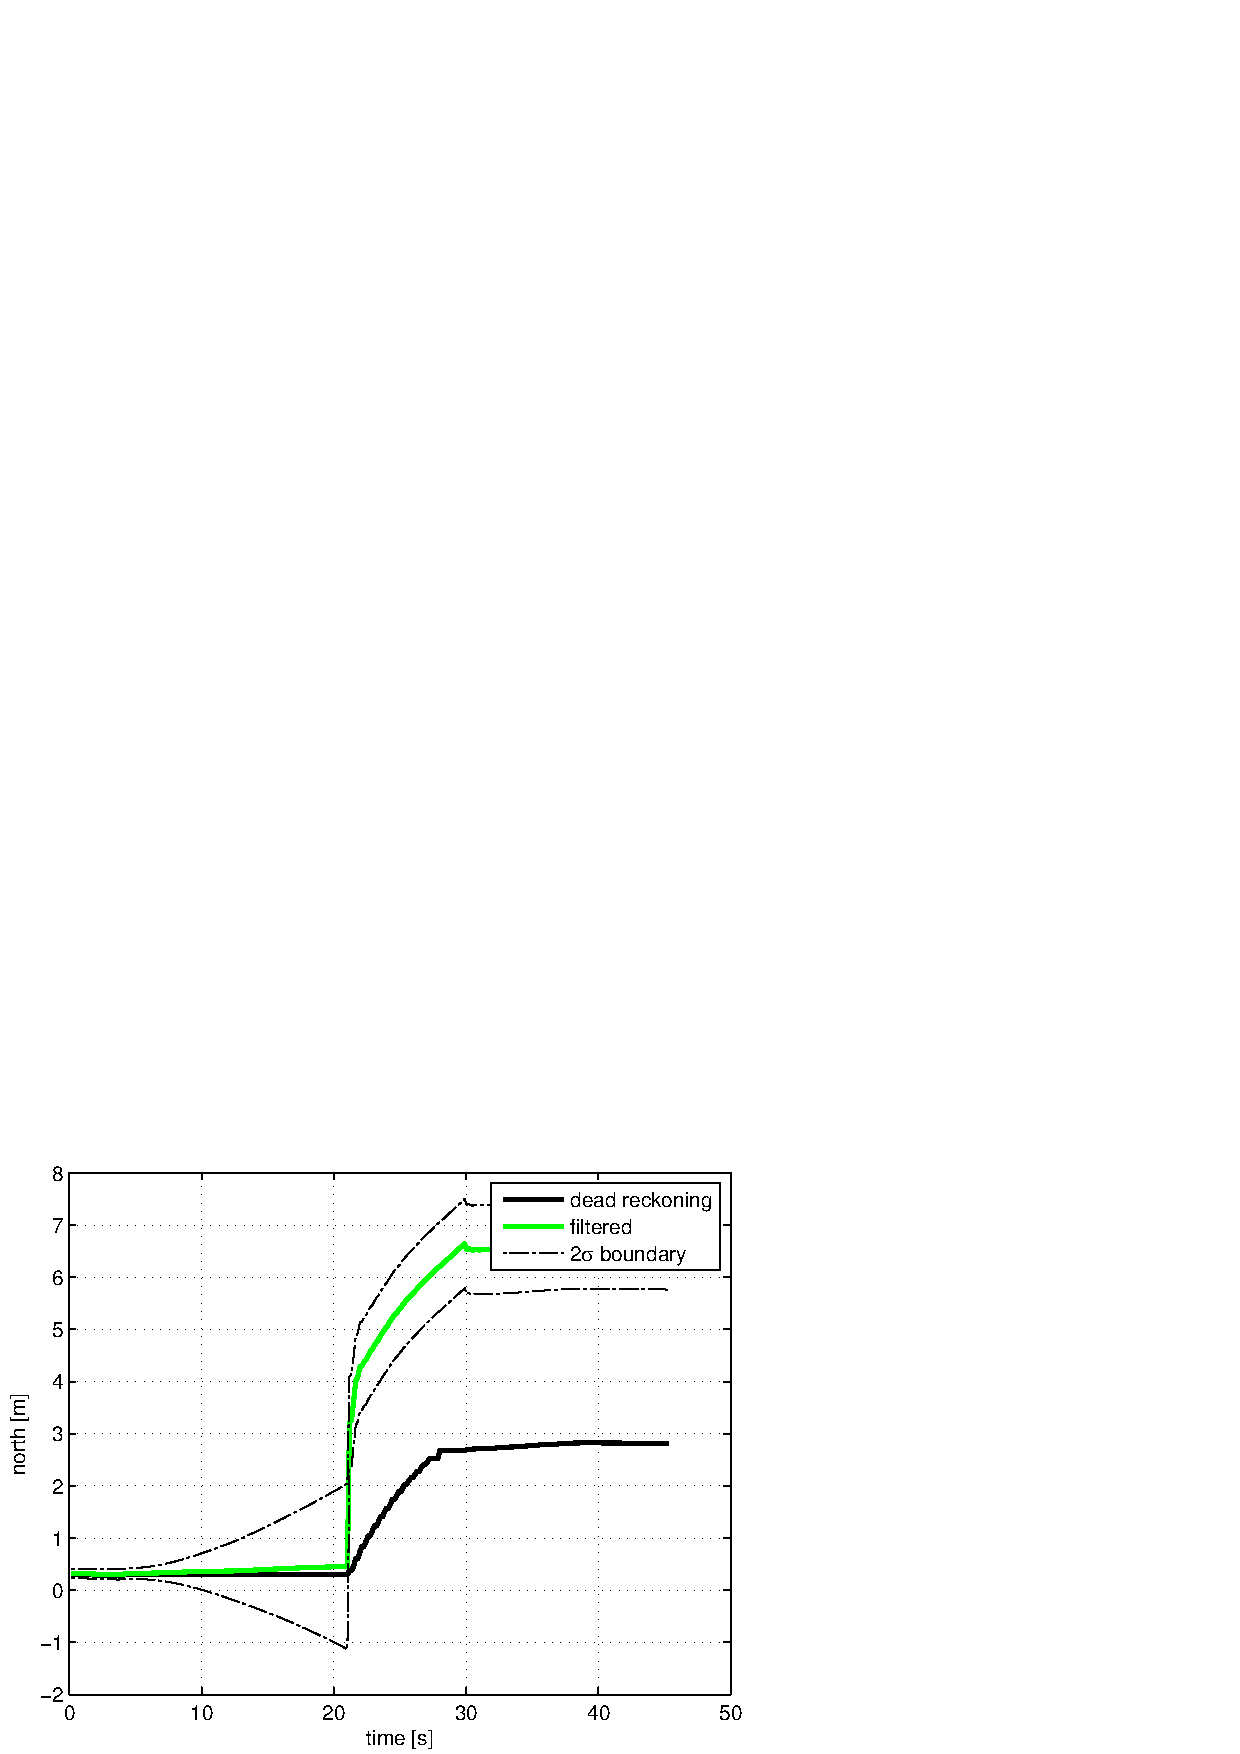
\includegraphics[width=0.49\linewidth]{fig/northLengthPool.pdf} 
			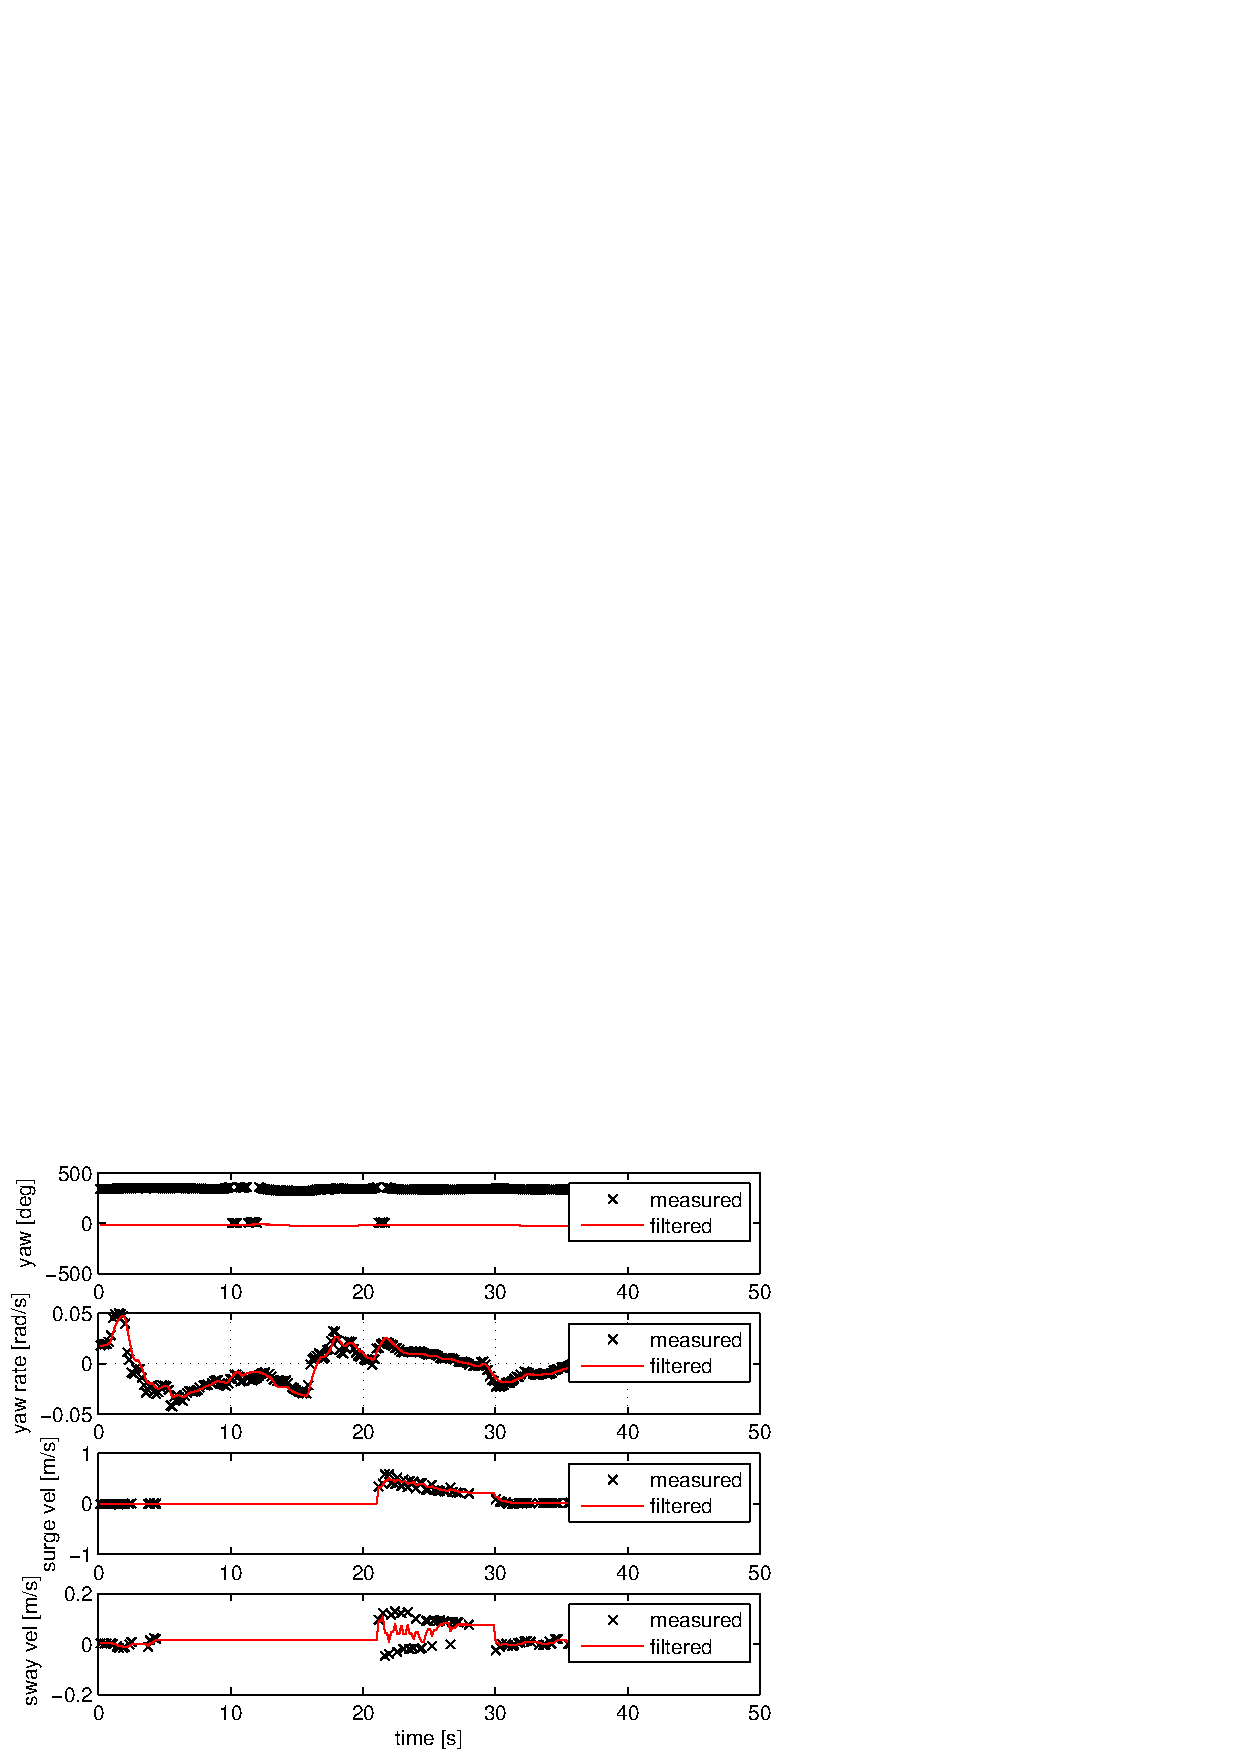
\includegraphics[width=0.49\linewidth]{fig/dynLengthPool.pdf}\\
			\textit{Outcome}: \pro less drift \\
			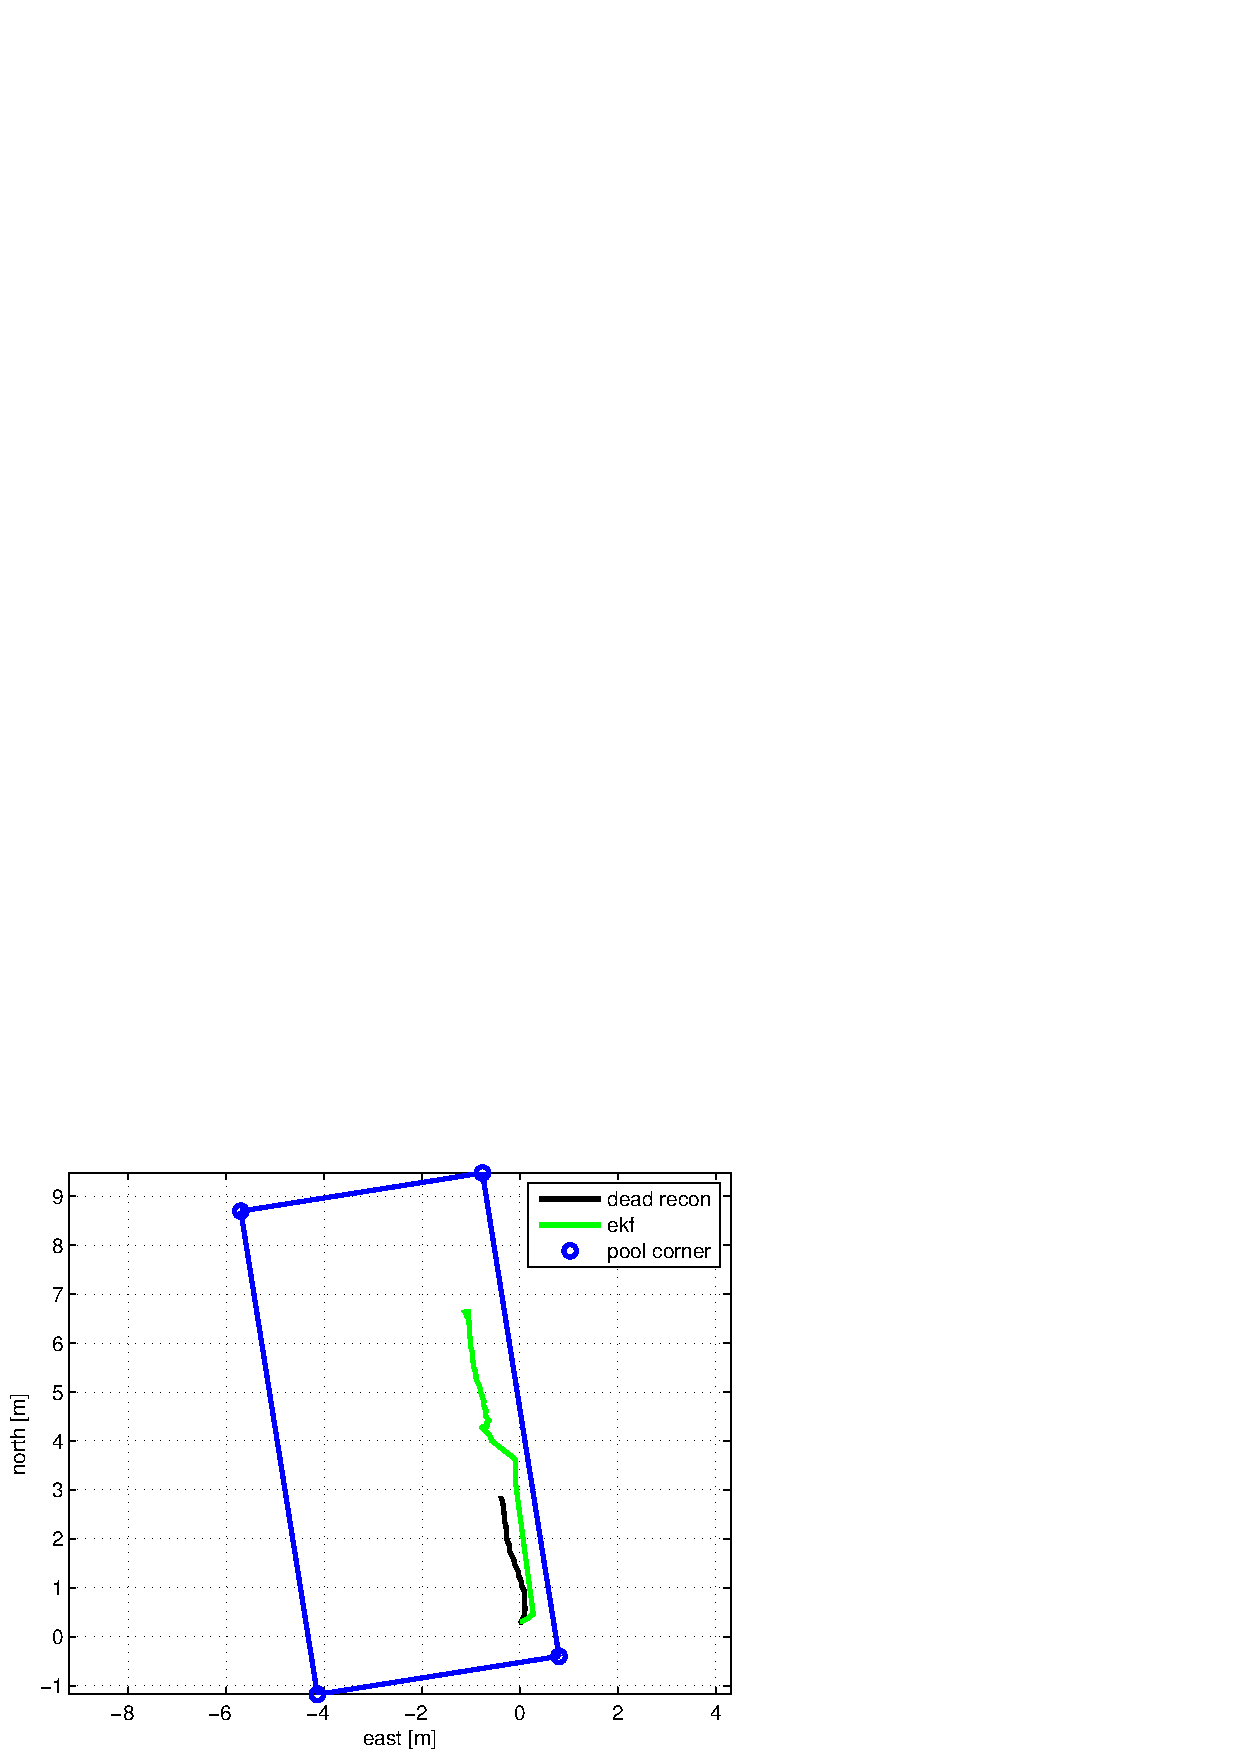
\includegraphics[width=0.5\linewidth]{fig/lengthPool.pdf}  \hspace{0.5em} 
			
\includegraphics[width=0.15\linewidth]{fig/path.pdf} 
\end{columns}
\textbf{III. Parametric Estimation: }
setting the values of model and observation noise covariance matrices dozes the ``trust'' in model/measurements. 
\end{frame}

%%%%%%%%%%%%%%%%%%%%%%%%%%%%%%%%%%%%%%%%%%%%%%%%%%%%%%%%%%%%%%%%%%%%%%%%%%%%%%%

\begin{frame}\frametitle{Performing Localisation in Real Missions}
\begin{block}{Spiral surfacing trajectory}
\begin{columns}
\column{.7\textwidth}
Spiral trajectory and surfacing action was taken with Nessie starting from the depth of around 12 m (Fig. ~\ref{fig:spiral}). %Trajectory seems to be smoother and less prone to drift . %Standard deviation of north and east measurement noise can be set 
\column{.28\textwidth}
\centering
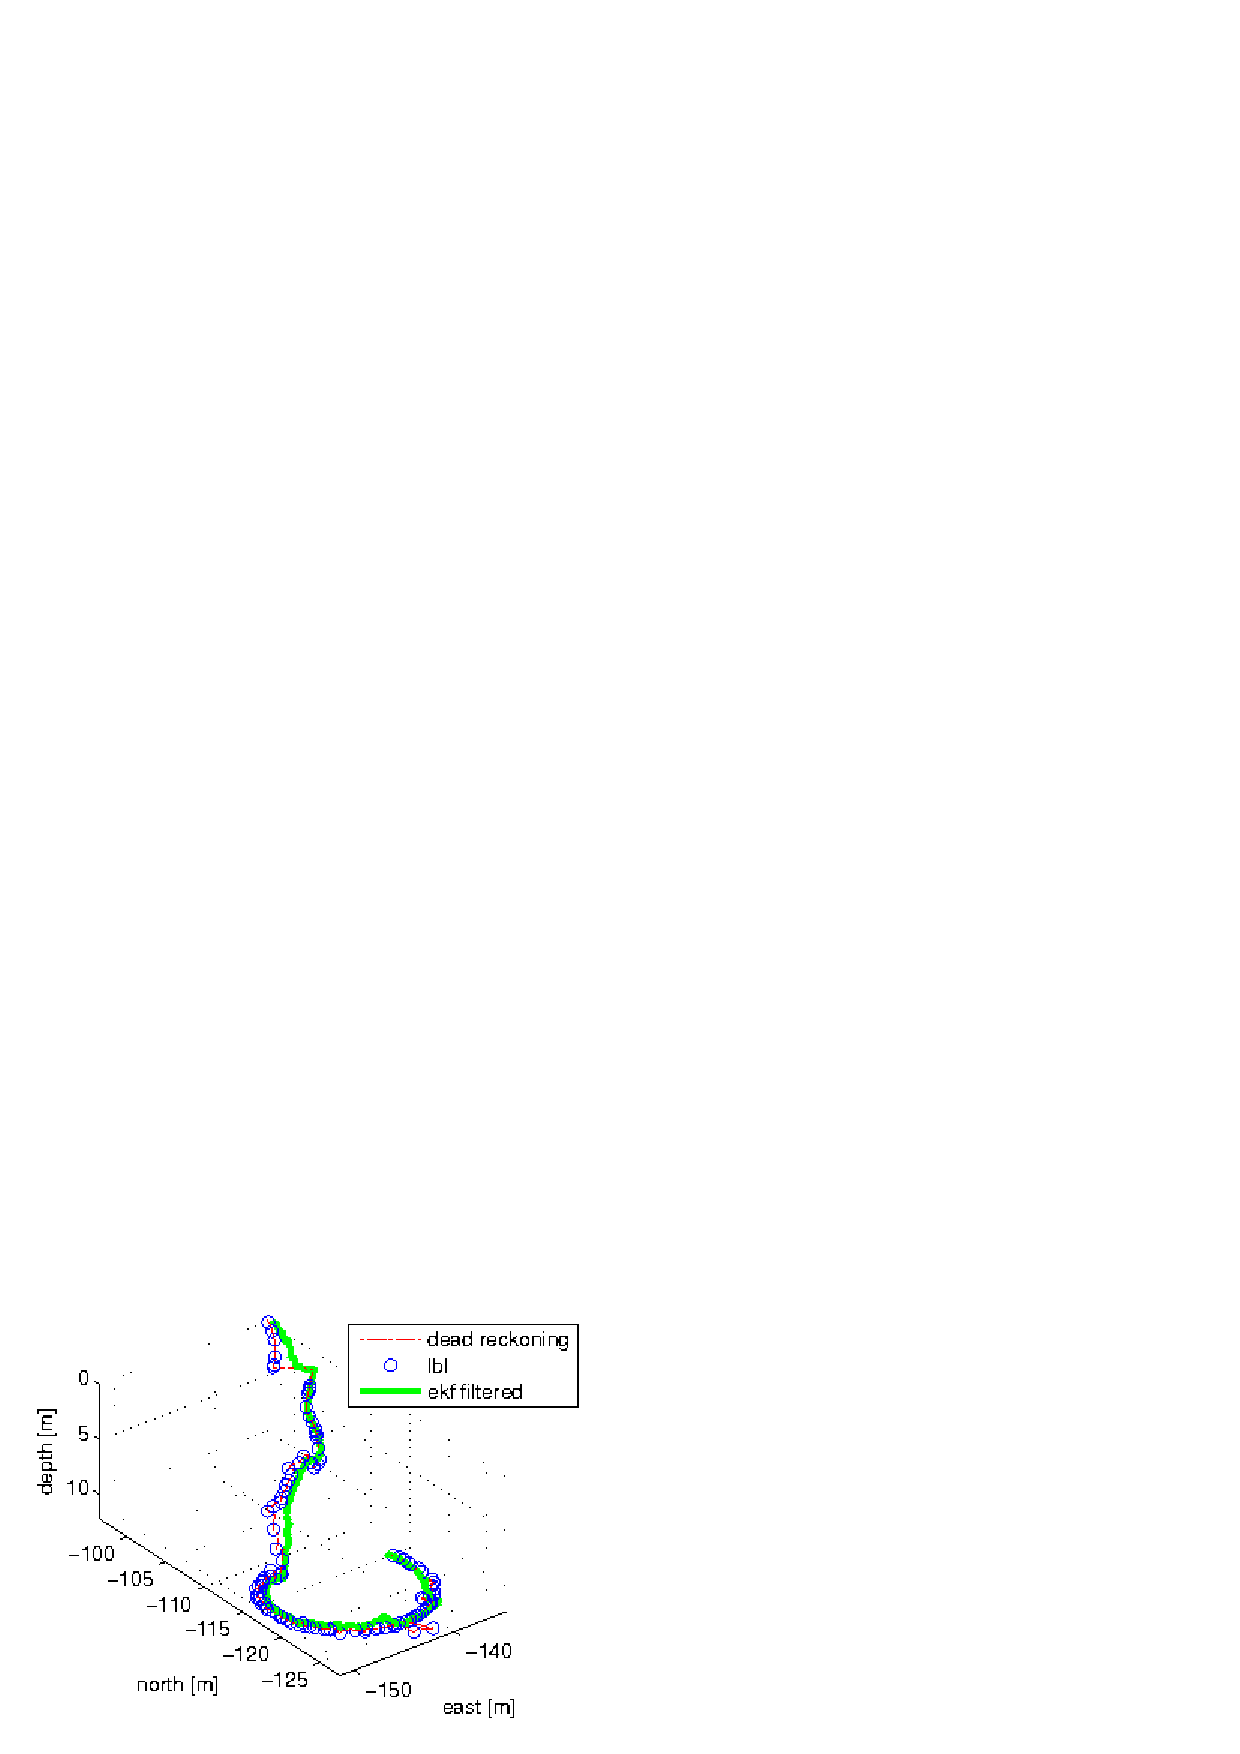
\includegraphics[width=0.7\linewidth]{fig/spiral3d.pdf}
\end{columns}
\end{block} 
\centering 
\begin{figure}
\vspace{-15pt}
\caption{Spiral trajectory localisation}
\vspace{-15pt}
\subfigure[{\scriptsize N/E localisation}]{\label{fig:ne2d}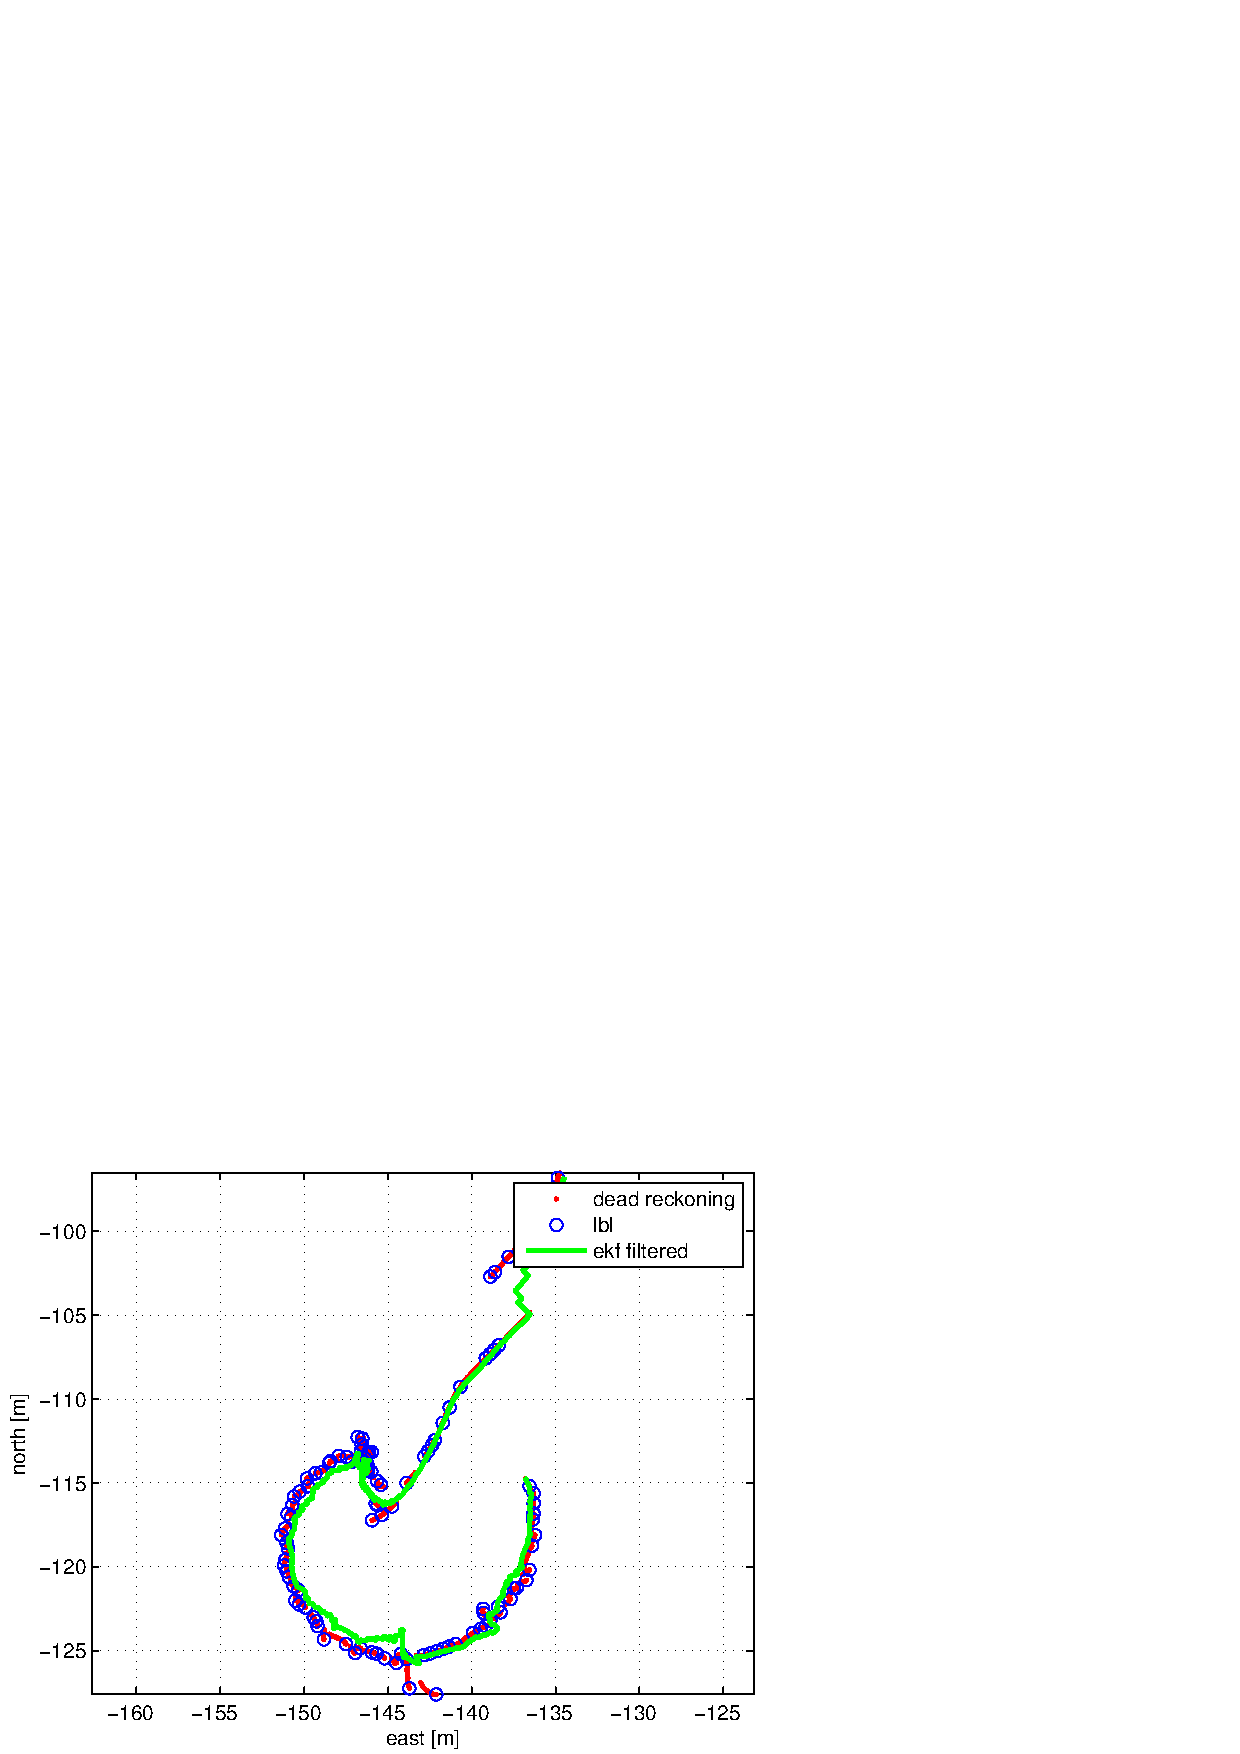
\includegraphics[width=0.45\linewidth]{fig/spiral2d.pdf}}
\subfigure[{\scriptsize depth filtering}]{\label{fig:depth}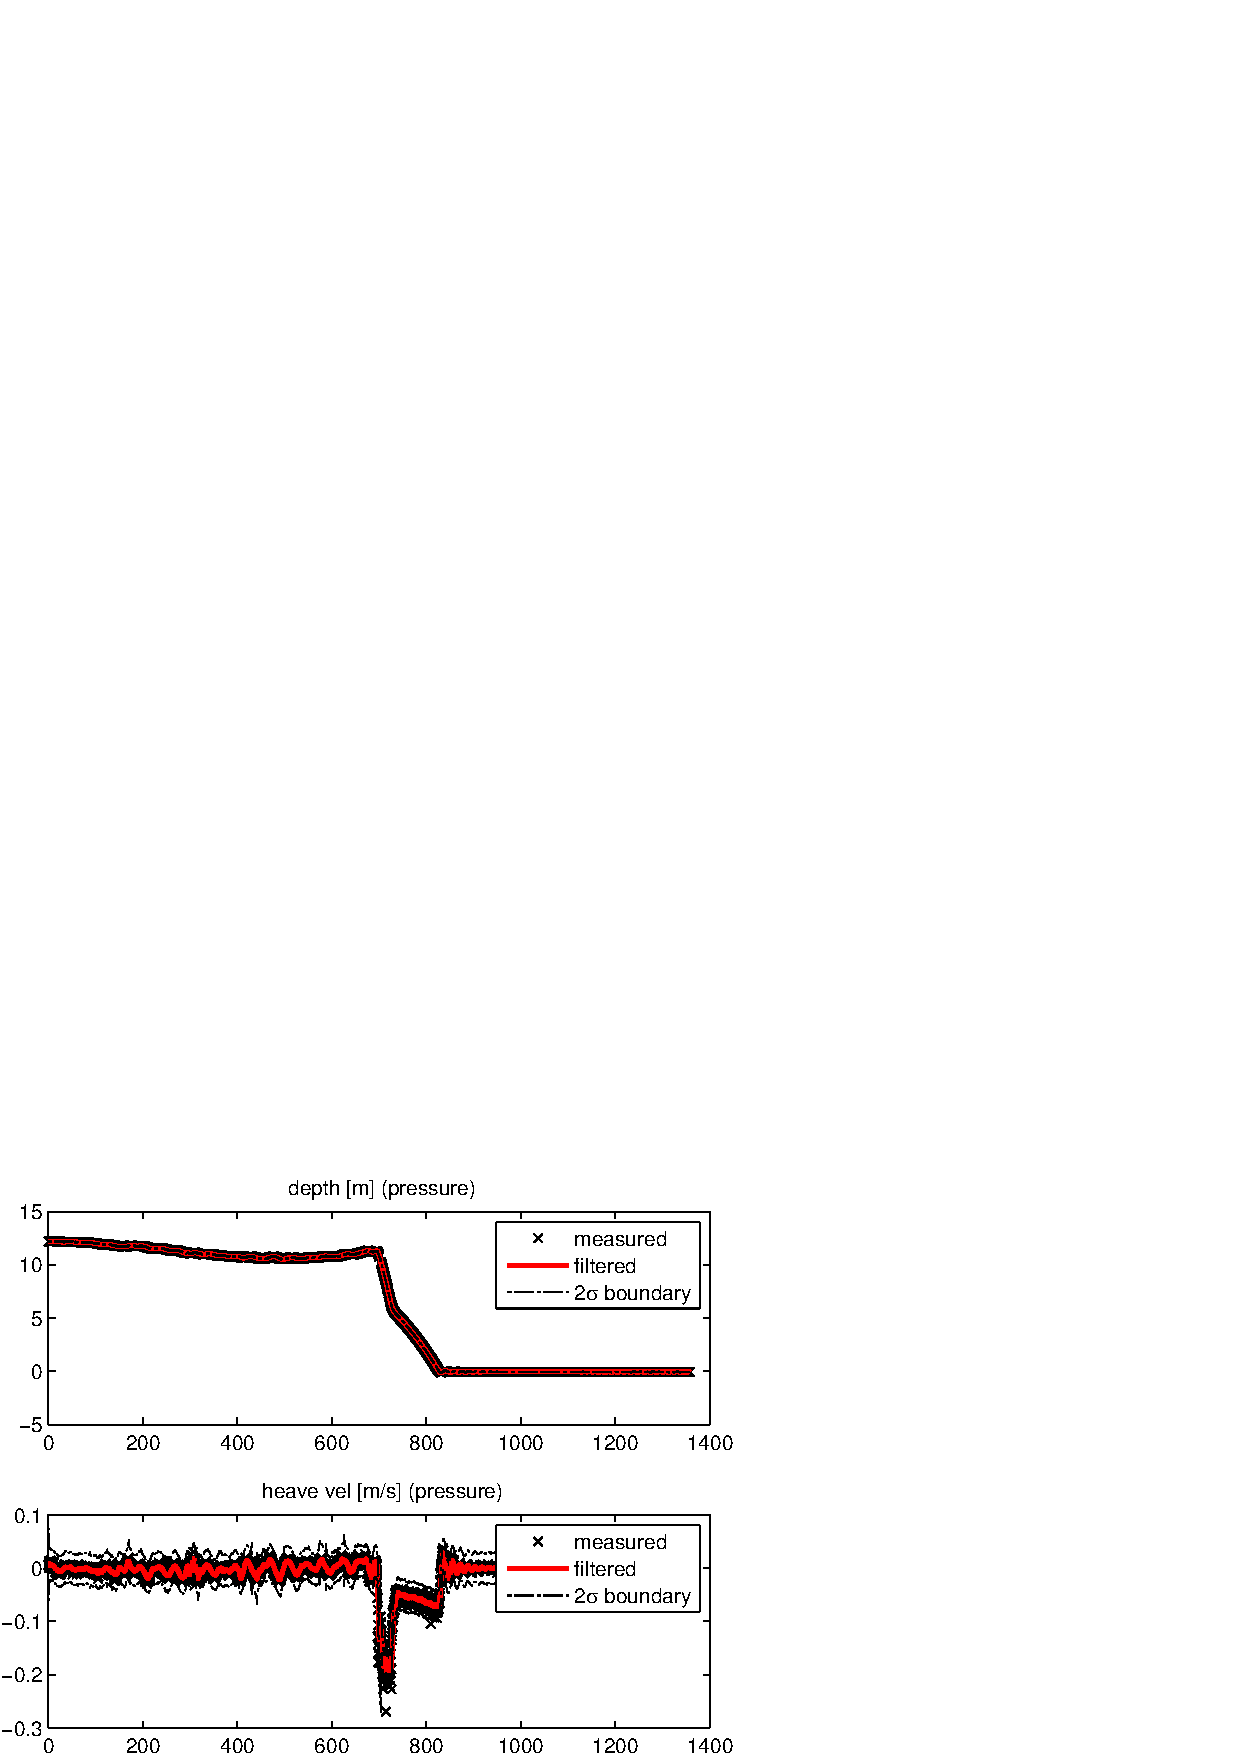
\includegraphics[width=0.45\linewidth]{fig/spiral-depth.pdf}} \\
\label{fig:spiral}
\end{figure}
%\begin{columns}[t]
%\column{.5\textwidth}
%\column{.2\textwidth}
\end{frame}

%%%%%%%%%%%%%%%%%%%%%%%%%%%%%%%%%%%%%%%%%%%%%%%%%%%%%%%%%%%%%%%%%%%%%%%%%%%%%%%


\begin{frame}\frametitle{AUV Localisation using EKF in Practise}
\vspace{-5pt}
\begin{block}{}
\center{\textbf{There is no is no exact ground truth for underwater robot localisation available}}
\end{block} 
\centering
Issues to Address in AUV Localisation%\end{center}
\begin{columns}[t]
\column{.36\textwidth}
{\centering \textbf{Heading Measurement}} \\
{\centering \hspace{6pt} \includegraphics[width=0.25\linewidth]{fig/tcm.pdf} \hspace{15pt} vs.
\includegraphics[width=0.25\linewidth]{fig/kvh.pdf}} \\
	\begin{columns}[t]
	\column{.55\linewidth}
	{\centering	
	Compass {\footnotesize(\textit{yaw})} } \\
	\contra \begin{footnotesize}prone to noise\end{footnotesize} \\
	\contra \begin{footnotesize}calibration\end{footnotesize} \\
	\pro    \begin{footnotesize}absolute\end{footnotesize}  \\ %  meas.	
		
	\column{.44\linewidth}
	{\centering	
	Gyro \\ {\footnotesize(\textit{yaw rate})} \\
	\pro    \begin{footnotesize}accurate\end{footnotesize}	\\
	\contra \begin{footnotesize}relative\end{footnotesize}  \\
	} %  meas.
	\end{columns}
\vspace{10pt}
Apart from being ``fused'', measurements of \textit{yaw rate} and \textit{yaw} can be taken with adjustable confidence. 	
\column{.3\textwidth}
{\centering \textbf{Nonlinearity}} \\
UKF \cite{julier96} is an interesting alternative in handling nonlinearities. 
\includegraphics[width=0.85\linewidth]{fig/UKFpipeTrack.pdf} \\
\pro {\footnotesize model emulation} \\
\pro {\footnotesize computational cost}
\column{.31\textwidth} % on filtering those outliers. (absolute position)
{\centering \textbf{LBL imprecision}} \\ %LBL measurements exhibit quite diverse range of values. 
Position updates can deviate from the trajectory, resulting in outliers. EKF was compared with median filter.  \\  
{\centering
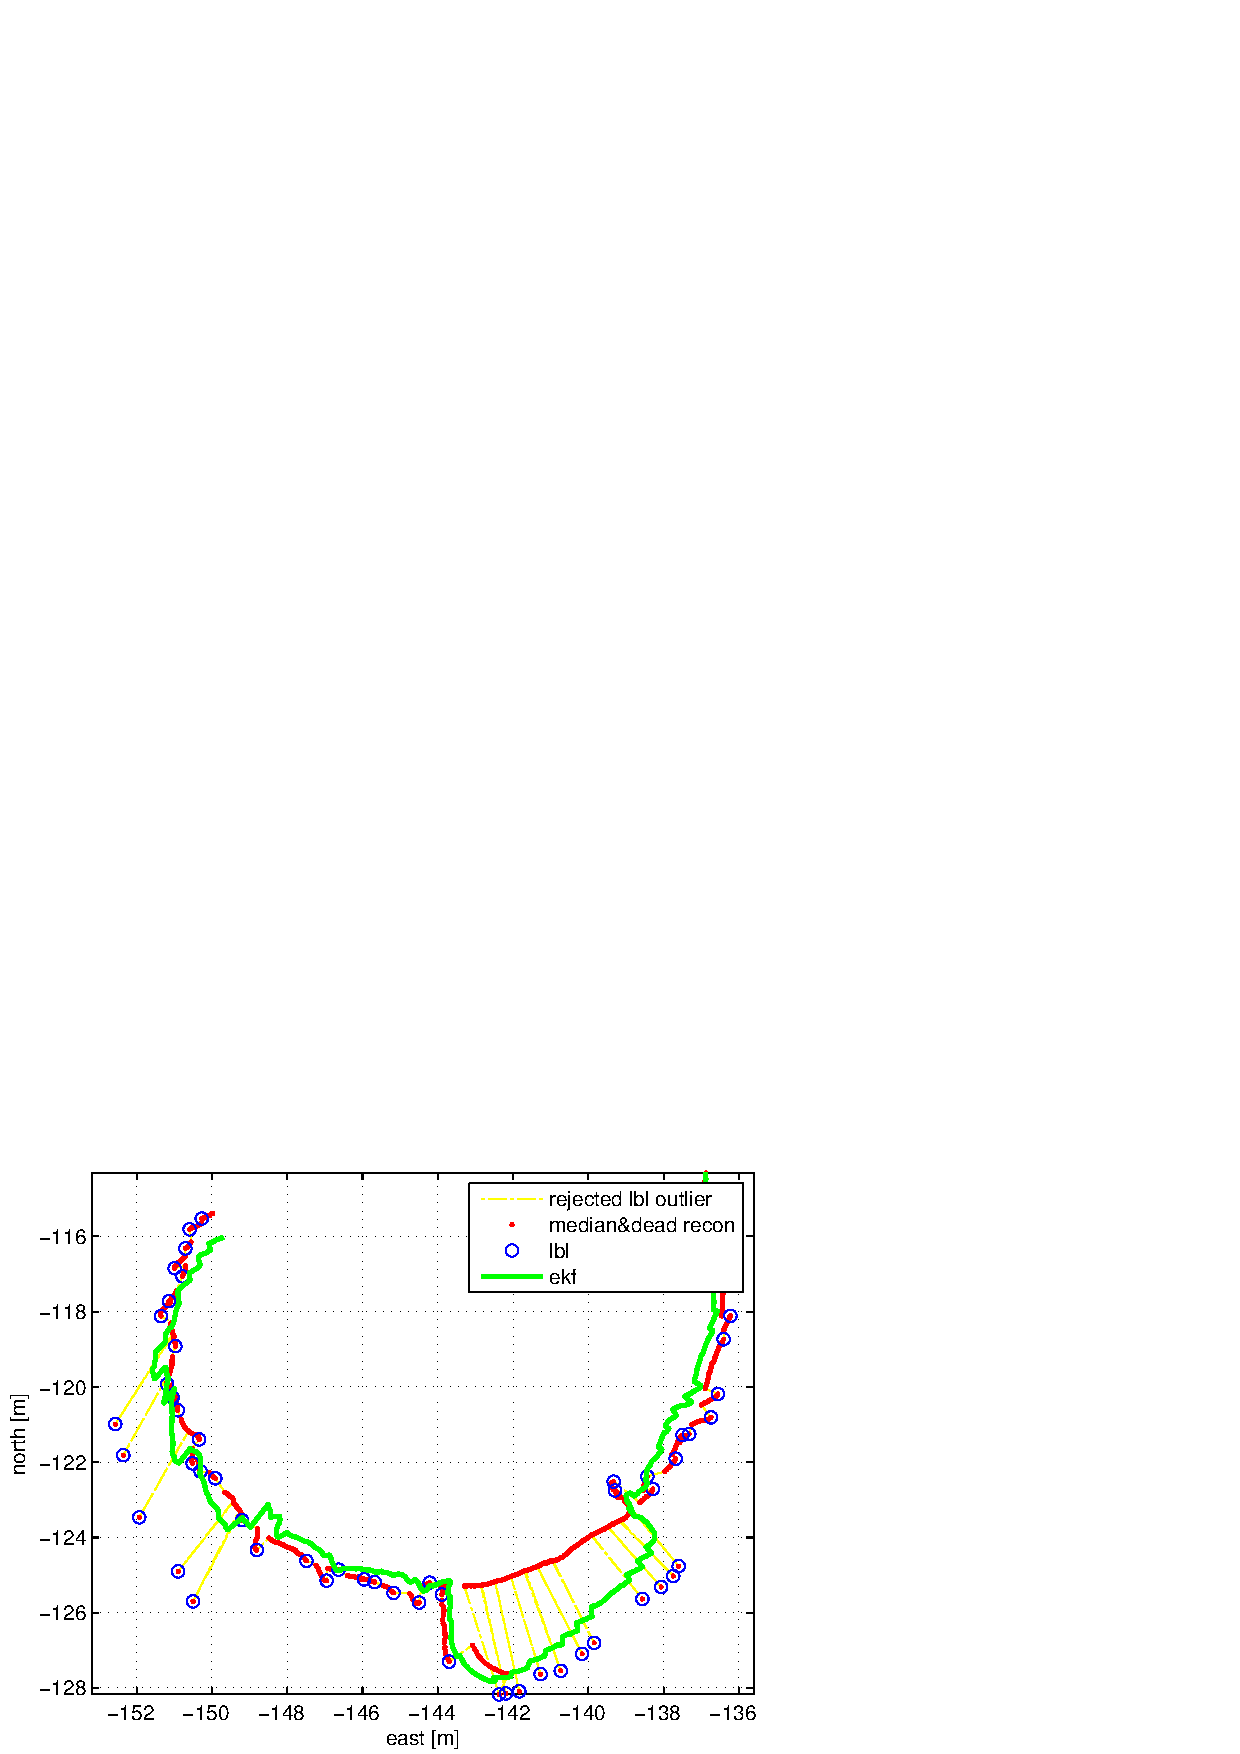
\includegraphics[width=0.8\linewidth]{fig/spiral-median-ekf.pdf} \\
\pro robust
} %outlier filtering 
\end{columns}
\end{frame}

%%%%%%%%%%%%%%%%%%%%%%%%%%%%%%%%%%%%%%%%%%%%%%%%%%%%%%%%%%%%%%%%%%%%%%%%%%%%%%%

\begin{frame}\frametitle{Performing Localisation in Real Missions}
\begin{block}{Rectangular trajectory in low depth}
\begin{columns}
\column{.78\textwidth}
Fairly noisy GPS signal (antenna is on the surface) was used as position correction. Parameters $\sigma_{north},\sigma_{east}$ of north and east measurement noise can be set (~\ref{fig:ne10}, ~\ref{fig:ne05}). Reasonably chosen values significantly correct the result obtained with pure dead reckoning. %Giving extremely high confidence with such amount of noise does not seem to be the best choice, however,
\column{.2\textwidth}
\centering
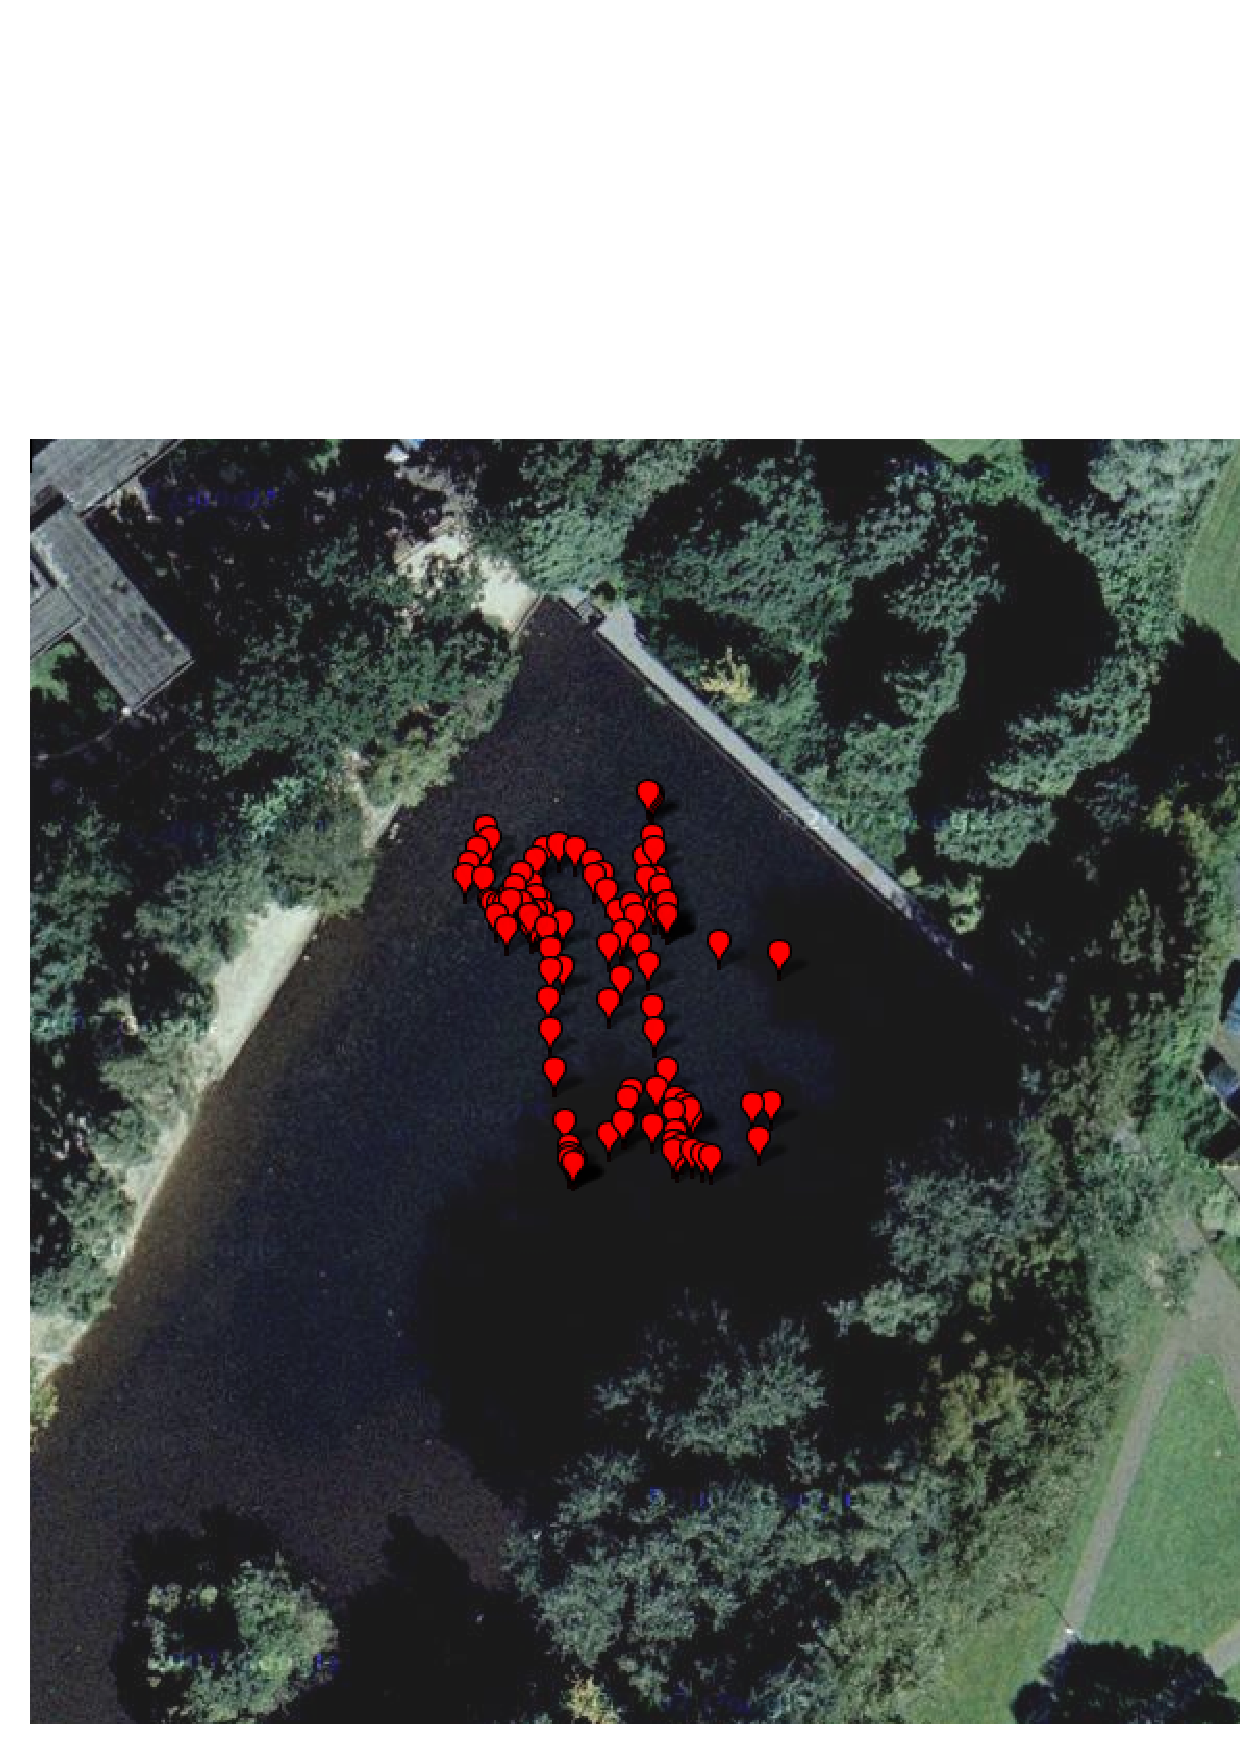
\includegraphics[width=0.95\linewidth]{fig/square-trajectory.pdf}
\end{columns}
\end{block}
\vspace{-10pt}
\centering 
\begin{figure}%(confidence in position measurement)  _{north}=\sigma_{east}  a_{north}=\sigma_{east}
\subfigure[{\scriptsize N/E localisation $\sigma= 1.0 m $}]{\label{fig:ne10} \includegraphics[width=0.32\linewidth]{fig/square10.pdf}} 
\subfigure[{\scriptsize N/E localisation $\sigma= 0.5 m $}]{\label{fig:ne05} \includegraphics[width=0.32\linewidth]{fig/square05.pdf} }
\subfigure[{\scriptsize Velocities \& heading}]{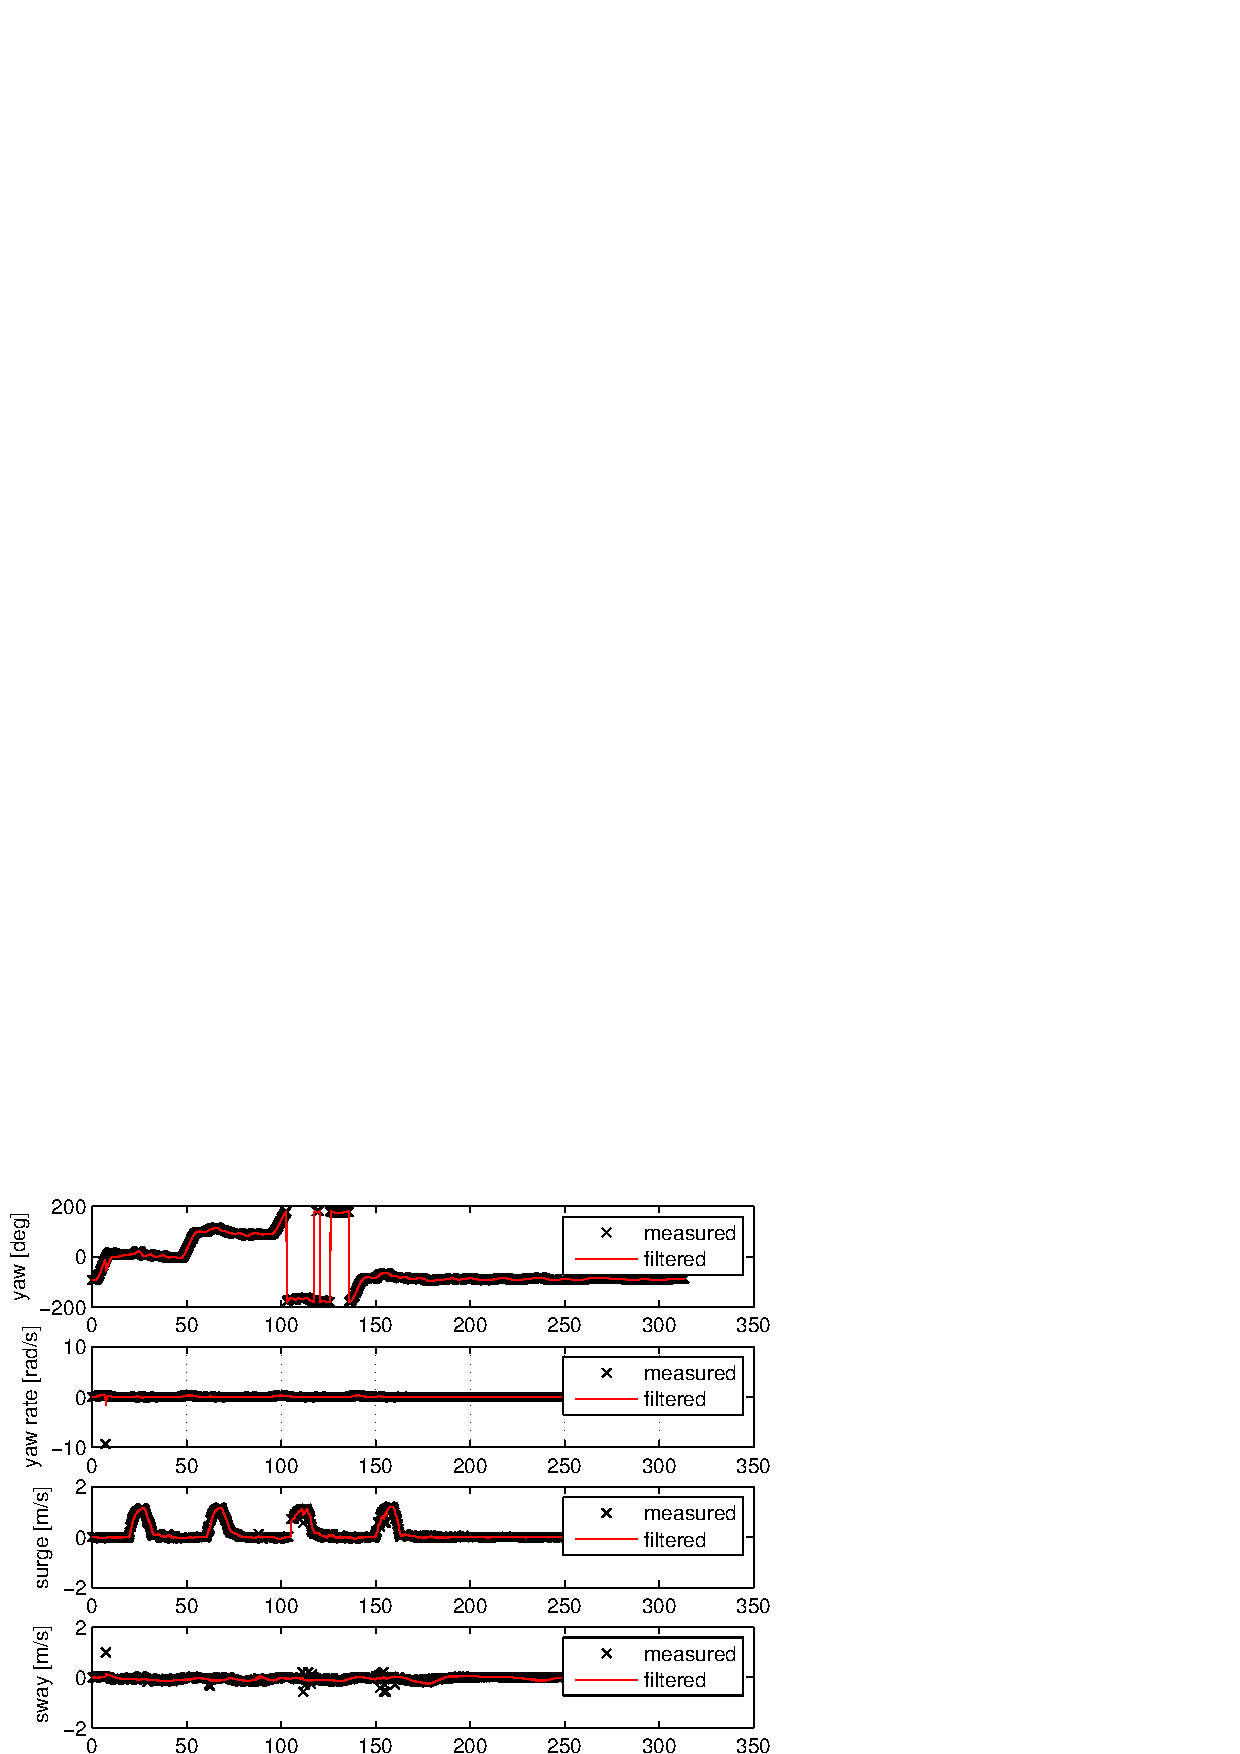
\includegraphics[width=0.3\linewidth]{fig/dynamics.pdf}}
\vspace{-10pt}
\caption{Rectangular trajectory localisation}
\vspace{-10pt}
\end{figure}
%From a noisy collection of position observations at the beginning, application of EKF with sensor fusion enabled having generally better performance in navigation.
\end{frame}

%%%%%%%%%%%%%%%%%%%%%%%%%%%%%%%%%%%%%%%%%%%%%%%%%%%%%%%%%%%%%%%%%%%%%%%%%%%%%%%

\begin{frame}\frametitle{Conclusions}
Presented work reports the design of an navigation module for a real AUV based on Extended Kalman Filter (EKF) .
\begin{itemize}
\item EKF proves to be useful navigation tool with satisfactory navigation performance and several convenient features: \\
{\scriptsize 
\hspace{0.5cm} capable of successfully combining together different sensory information (\textit{sensor fusion}) \\
\hspace{0.5cm} estimate that tends to be optimal with respect to set expectations \\
\hspace{0.5cm} recovering from the missing measurements \\
\hspace{0.5cm} filtering corrupted position information: outliers or signal noise \\
}
%EKF is a great tool since it tries to satisfy the set uncertainty boundaries and fuse all the available information trying to make the most out of it combined together in one mathematical system. %- ``filtration with semantics''
%\\
\item 5DOF \textit{constant velocity} mathematical model for state prediction was introduced 
%\\ One of the issues that were addressed was the s
\item Suitable management of heading measurement was addressed and the role of EKF in correcting deficiencies
%\\
%\item Sensor fusion was explored as mean of improving the estimation
%\\
\item Nonlinearity issues have been investigated with the usage of Unscented Kalman Filter (UKF)
\end{itemize} 
\end{frame}

%%%%%%%%%%%%%%%%%%%%%%%%%%%%%%%%%%%%%%%%%%%%%%%%%%%%%%%%%%%%%%%%%%%%%%%%%%%%%%%

\begin{frame}\frametitle{Future Work}
\begin{itemize}
\item More trials, particularly ones where the vehicle trajectory has been fixed to known landmarks so that the results of localisation could be thoroughly evaluated with trustful ground truth
%
% \\
%{\scriptsize 
%\hspace{0.5cm} capable of successfully combining together different sensory information (\textit{sensor fusion}) \\
%\hspace{0.5cm} estimate that tends to be optimal with respect to set expectations \\
%\hspace{0.5cm} recovering from the missing measurements \\
%\hspace{0.5cm} filtering corrupted position information, outliers, or signal noise \\
%}
%EKF is a great tool since it tries to satisfy the set uncertainty boundaries and fuse all the available information trying to make the most out of it combined together in one mathematical system. %- ``filtration with semantics''
%\\
\item Navigation of the tilted vehicle movements in order to make an evaluation of the influence of the 5th d.o.f

%\\ One of the issues that were addressed was the s
\item EKF could be improved so that it works with control inputs
%\\
%\item Sensor fusion was explored as mean of improving the estimation
%\\
\item Filtering of the noisy absolute position gives space for improvement. Solution for rejecting outliers could rely on some version of \textit{back-filtering} - filtering based on history of received observations.% since the measured position tends to be quite uncertain and prone to different sorts of noise. 


\end{itemize} 
\end{frame}

%%%%%%%%%%%%%%%%%%%%%%%%%%%%%%%%%%%%%%%%%%%%%%%%%%%%%%%%%%%%%%%%%%%%%%%%%%%%%%%
%\begin{frame}
%\frametitle{Kalman fusion strategy}
%Describe the algorithm used.
%\end{frame}
%%%%%
%\begin{frame}
%\frametitle{Localisation algorithm}
%Describe the algorithm used and the ones that were tested.
%\end{frame}
%%%%%
%\begin{frame}
%\frametitle{Graphical results}
%2d plots of some missions.
%Experimental results in real environment presented.
%\end{frame}
%%%%%%%%%%%%%%%%%%%%%%%%%%%%%%%%%%%%%%%%%%%%%%%%%%%%%%%%%%%%%%%%%%%%%%%%%%%%%%%

%\begin{frame} \frametitle{Results Accuracy of the system}
- usage of two different heading sources
- error wrt to distance

Interpretation of the results.
\end{frame}

%%%%%%%%%%%%%%%%%%%%%%%%%%%%%%%%%%%%%%%%%%%%%%%%%%%%%%%%%%%%%%%%%%%%%%%%%%%%%%%
%\begin{frame}[fragile] % Notice the [fragile] option beside \begin{frame} %
%\frametitle{Verbatim}
%\begin{example}[Putting Verbatim]
%\begin{verbatim}
%\begin{frame}
%\frametitle{Outline}
%\begin{block}
%{Why Beamer?}
%Does anybody need an introduction to Beamer?
%I don't think so.
%\end{block}
%\end{frame}\end{verbatim} % Extra carriage return causes problem wit verbatim %
%\end{example}
%\end{frame}

%%%\begin{frame}[fragile]  % notice the fragile ooption, since the body
%%%			% contains a verbatim command
%%%Example of the \verb|\cite| command to give a reference is below:
%%%
%%%With an example of citation, \cite{ribas10}, we may proceed to the Bibliograhy section.
%%%\end{frame}

\begin{frame}
\frametitle{References}
\footnotesize{
\begin{thebibliography}{99}

%      \bibitem{ribas10} 
%      D. Ribas, P. Ridao, and J. Neira.
%      \newblock {U}nderwater {S}lam for {S}tructured {E}nvironments using an {I}maging {S}onar
%      \newblock {\em Springer Verlag, 2010}

 \bibitem{ribas10} D. Ribas, P. Ridao, and J. Neira. (2010)
 \newblock {U}nderwater {S}lam for {S}tructured {E}nvironments using an {I}maging {S}onar. \newblock \emph{\em Springer Verlag} 
%  
 
 \bibitem{julier96} Julier, S. and Uhlmann, J.K. (1996)
 \newblock {A} general method for approximating nonlinear transformations of probability distributions.
 \newblock \emph{\em Robotics Research Group, Department of Engineering Science, University of Oxford}
 
 \bibitem{thrun05}  S. Thrun, W. Burgard, and D. Fox. (2005)
 \newblock {P}robabilistic robotics
 \newblock {\em MIT Press}	
 
 \bibitem{grewal01} Grewal, M.S. and Andrews, A.P. (2001)
 \newblock {K}alman filtering: theory and practice using MATLAB.
 \newblock {\em Wiley Online Library}
  
 \bibitem{ristic04} Ristic, B. and Arulampalam, S. and Gordon, N. (2004)
 \newblock {B}eyond the Kalman filter: Particle filters for tracking applications.
 \newblock {\em Artech House Publishers}

% \bibitem{farrell98} Jay Farrell and Jay A. Farrell (1998)
% \newblock {T}he Global Positioning System \& Inertial Navigation.
% \newblock {\em McGraw-Hill Professional} 
       
\end{thebibliography}
}
\end{frame}

\begin{frame}
\centerline{The End}
\end{frame}


% End of slides
\end{document} 